\section{Simulated Camera Calibration}
\label{section:camera_calibration}

As described in Section \ref{subsection:setup_and_tools}, a standard Gazebo ROS camera sensor is ``mounted'' to the Iris' gimbal and provides a simulated camera image as a ROS topic. The important aspects of this code are the specifications for the camera's distortion coefficients, which are all set to 0.0. Any library using a camera for image processing will require these values. Instead of passing these values to the WhyCon and April Tag libraries directly, the \texttt{calibrate\_camera} ROS module was used to generate a \texttt{.yaml} file containing the empirically determined values. This method is a de facto standard way of calibrating a camera in ROS, and can be used during migration to a physical system.
% \begin{lstlisting}[style=XML,caption={Instantiation of a Gazebo ROS camera sensor.},captionpos=b,label={lst:camera_sensor_instantiation}]
% <plugin name="camera_controller" filename="libgazebo_ros_camera.so">
%     <alwaysOn>true</alwaysOn>
%     <updateRate>0.0</updateRate>
%     <robotNamespace>/</robotNamespace>
%     <cameraName>camera</cameraName>
%     <imageTopicName>image_raw</imageTopicName>
%     <cameraInfoTopicName>camera_info</cameraInfoTopicName>
%     <frameName>camera_link</frameName>
%     <distortionK1>0.0</distortionK1>
%     <distortionK2>0.0</distortionK2>
%     <distortionK3>0.0</distortionK3>
%     <distortionT1>0.0</distortionT1>
%     <distortionT2>0.0</distortionT2>
% </plugin>
% \end{lstlisting}
%<hackBaseline>0.07</hackBaseline>
The \texttt{calibrate\_camera} script requires a rectangular ``chessboard'' defined by $m-1$ and $n-1$ where $m$ is the amount of squares along one side, and $n$ is the amount of squares along a perpendicular side. This chessboard was inserted into \texttt{sandbox.world} as a texture, as shown in Figure \ref{fig:camera_calibration}. The sizes of the squares in the chessboard are an important factor in calibration, and they were approximately the size of a single 1-meter grid square. The drone was directed around the chessboard in order to view it from many angles and distances, after which a calibration file was generated.

\begin{figure}[ht]
    \begin{subfigure}[b]{0.48\textwidth}
        \centering
        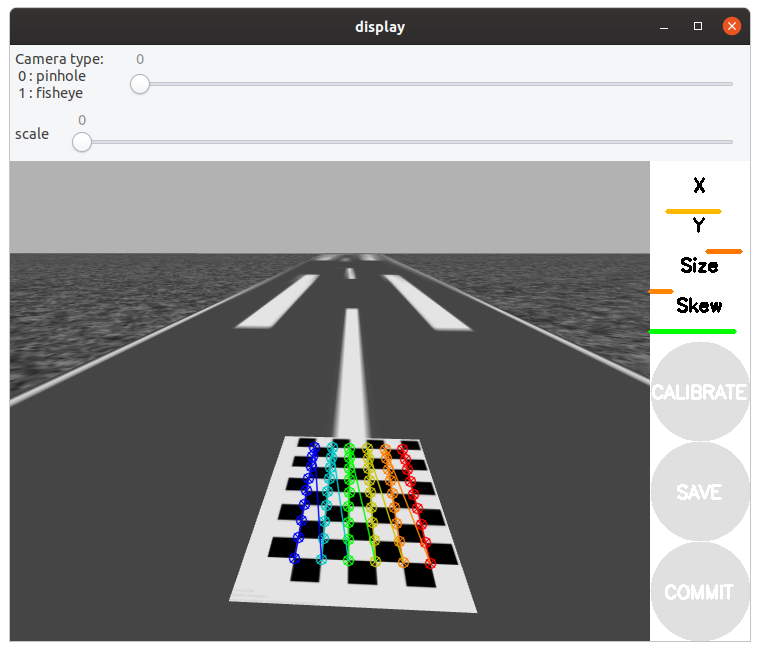
\includegraphics[height=5cm]{images/calibration_camera_view.png}
        \caption{``Chessboard'' detection.}
        \label{subfig:calibration_camera_view}
    \end{subfigure}
    \begin{subfigure}[b]{0.48\textwidth}
        \centering
        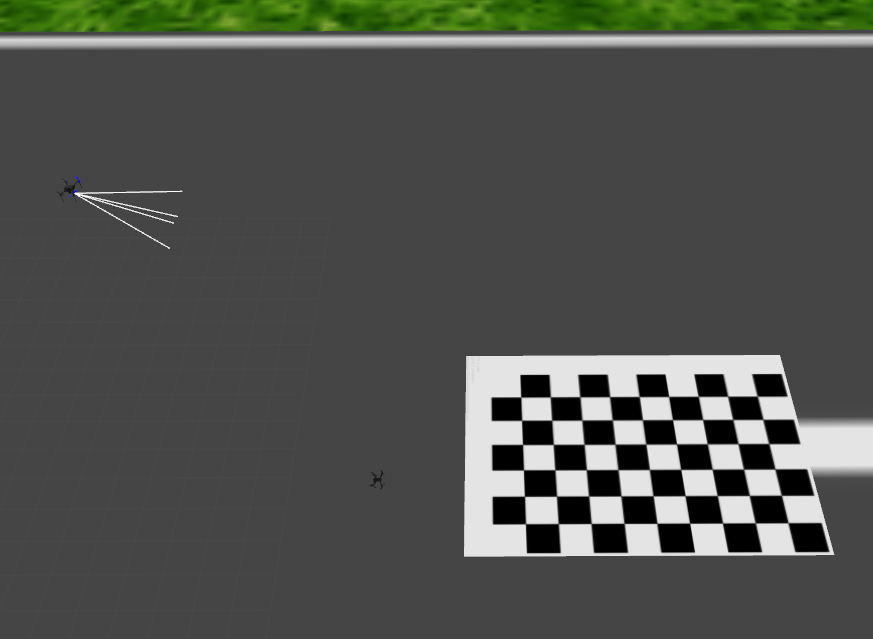
\includegraphics[height=5cm]{images/calibration_birds_eye_view.png}
        \caption{The calibration ``chessboard'' from above.}
        \label{subfig:calibration_birds_eye_view}
    \end{subfigure}
    \caption{Calibration of the simulated camera.}
    \label{fig:camera_calibration}
\end{figure}

The calibration generated the following data which has been rounded for conciseness. The camera intrinsics matrix $K$ contains $f_x, f_y$ which are the focal lengths of the camera in the $x$ and $y$ dimensions respectively, in pixel units. It also contains $c_x, c_y$ which represent the coordinates of a principal point that should be near the image center. After calibration, the simulated camera sensor is calculated to have focal lengths $f_x, f_y$ of 398.2 and 390.8 pixels respectively. With a resolution of 640x480 pixels, the calibrated values of $c_x=299.9$ and $c_y=227.5$ are only \textit{near} the image center - slightly to the upper left.

\begin{equation}
    K=
    \begin{pmatrix}
        f_x & 0 & c_x\\
        0 & f_y & c_y\\
        0 & 0 & 1
    \end{pmatrix}
    =
    \begin{pmatrix}
        398.2 & 0 & 299.9\\
        0 & 390.8 & 227.5\\
        0 & 0 & 1
    \end{pmatrix}
    \label{equation:camera_intrinsic_matrix}
\end{equation}

The distortion coefficients determined by the camera calibration, $D_T$, are roughly equivalent to those set in the camera plugin's parameters. The radial distortion coefficients $k_1, k_2, k_3$ are set to exactly zero but are calculated as only near-zero after the calibration. The tangential distortion coefficients $p_1, p_2$, corresponding to T1 and T2 in the camera plugin parameters, are also non-zero but near-zero.

\begin{equation}
    D^T=
    \begin{pmatrix}
        k_1\\k_2\\p_1\\p_2\\k_3
    \end{pmatrix}
    =
    \begin{pmatrix}
        0.0576\\-0.0321\\0.0041\\-0.0203\\0
    \end{pmatrix}
    \label{equation:distortion_coefficients}
\end{equation}

It is important to note that the process of calibrating the camera module has been developed out of necessity because typical real world cameras have non-negligible distortion coefficients. The values determined for $D^T$ are significantly lower in magnitude than those of a typical, real camera. 

% The rotation matrix $R$ determines the rotation between the first and second cameras in a stereo-vision setup. In this monocular case, the rotation is 

% \begin{equation}
%     R=
%     \begin{pmatrix}
%         1 & 0 & 0\\
%         0 & 1 & 0\\
%         0 & 0 & 1
%     \end{pmatrix}
%     \label{equation:rectification_matrix}
% \end{equation}

% \begin{equation}
%     P=
%     \begin{pmatrix}
%         406.9 & 0 & 282.8 & 0\\
%         0 & 412.1 & 229.92 & 0\\
%         0 & 0 & 1 & 0
%     \end{pmatrix}
%     \label{equation:projection_matrix}
% \end{equation}


\section{Gimbal Controller}
\label{section:gimbal_controller_results}

As stated in Section \ref{subsection:aiming_the_camera}, the main job of the gimbal controller is to aim the camera directly at the landing platform. It does this by using 2 PID controllers - one on its pitch angle and one on its yaw angle - to control its 2 degrees of freedom. Initially, PD controllers were used for this purpose, but they were inadequate as the simulated gimbal has spring forces which tend to keep the gimbal's positions at their original points. As the magnitude of the pitch or yaw angles increases, the force required to further increase the angle's magnitude increases. Over time, a small integral gain helps correct the error caused by this change in required force. Table \ref{tab:gimbal_controller_pid_gains} shows the gains for the gimbal PID controllers.

\begin{table}[ht]
    \centering
    \begin{tabular}{|c|c|c|c|}
    \hline
        Controller & $k_p$ & $k_i$ & $k_d$ \\\hline
        Pitch & 0.25 & 0.1 & 0.025 \\\hline
        Yaw & 0.25 & 0.1 & 0.025 \\\hline
    \end{tabular}
    \caption{Gimbal controller PID gains.}
    \label{tab:gimbal_controller_pid_gains}
\end{table}

The $x$ and $y$ components of the un-transformed landing platform pose comprise the input for target angle calculation, and these target angles are used as the set points for the PID controllers. The $x$ and $y$ components are scaled by a factor inversely proportional to the $z$ component in order to allow the PID controllers to function in a stable way over a variety of distances. If the $x$ and $y$ components are used without scaling, the PID controllers wildly overshoot at long distances and undershoot at short distances. Figures \ref{subfig:x_displacement} and \ref{subfig:y_displacement} show the performance of the gimbal controller during 10 landings. In both figures, each line represents a single attempt to aim camera over the course of the landing. Time $t=0$ represents that time of first recognition of the landing platform. At about 30 seconds in each landing sequences, the drone has made contact with the landing platform. The graph continues in time until the drone disarms, completing the landing. Figure \ref{subfig:x_displacement} shows that, after some oscillation, the yaw of the gimbal is adjusted so that the marker is in the center of the camera's view in the $x$ direction. Figure \ref{subfig:y_displacement} shows similar results with regards to the gimbal's pitch, but with an added, temporary bias during which time the gimbal is pointed slightly lower than the landing platform. This is because, when the drone is close to the landing pad, the April Tag marker is almost directly in front of the drone and therefore the spring resistance in the gimbal is high. The error is eventually corrected by the integral gain and the marker becomes centered in the $y$ direction of the camera frame. Centering of the landing platform in the camera's field of view is represented by the convergence of each line to 0. However, even though the ideal goal of the gimbal controller is to keep the landing platform centered in this way, it is only critical that it must keep the landing platform in the camera's field of view throughout a variety of orientations and displacements. These figures show that the gimbal controller does accomplish this goal.

\begin{figure}[ht]
    \centering
    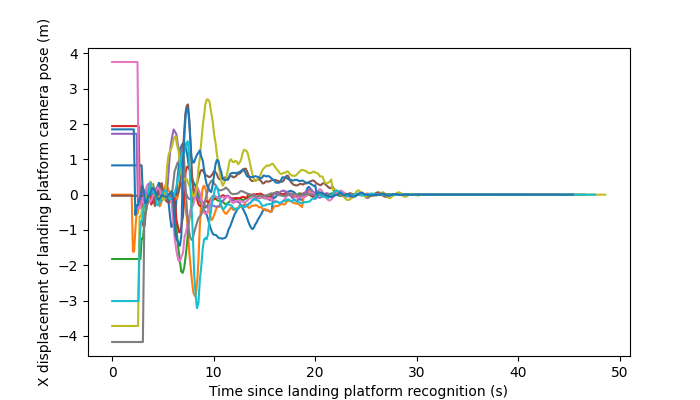
\includegraphics[width=0.7\textwidth]{images/x_displacement.png}
    \caption[Landing platform $x$ displacement in camera frame versus time.]{Landing platform $x$ displacement in camera frame versus time. Each line represents a single attempt to aim the camera during landing.}
    \label{subfig:x_displacement}
\end{figure}

\begin{figure}[ht]
    \centering
    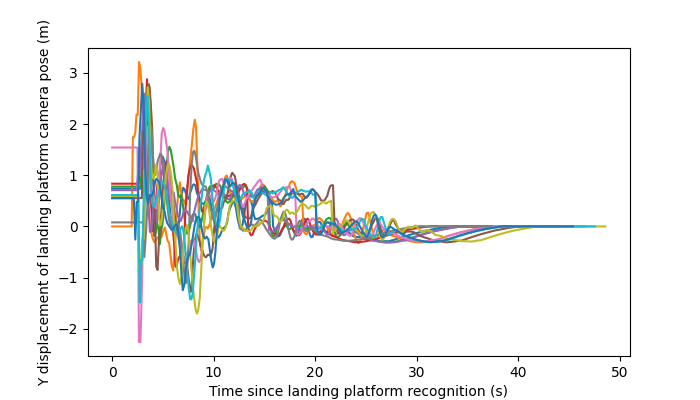
\includegraphics[width=0.7\textwidth]{images/y_displacement.png}
    \caption[Landing platform $y$ displacement in camera frame versus time.]{Landing platform $y$ displacement in camera frame versus time. Each line represents a single attempt to aim the camera during landing.}
    \label{subfig:y_displacement}
\end{figure}

% \begin{figure}[ht]
%     \centering
%     \begin{subfigure}[b]{0.47\textwidth}
%         \centering
%         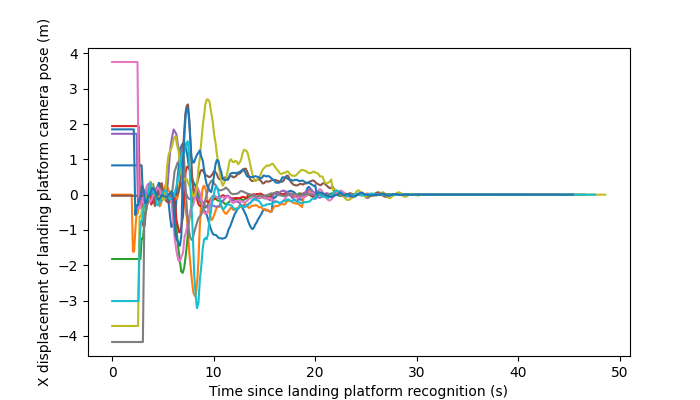
\includegraphics[width=\textwidth]{images/x_displacement.png}
%         \caption{Landing platform X displacement in camera frame.}
%         \label{subfig:x_displacement}
%     \end{subfigure}
%     \begin{subfigure}[b]{0.47\textwidth}
%         \centering
%         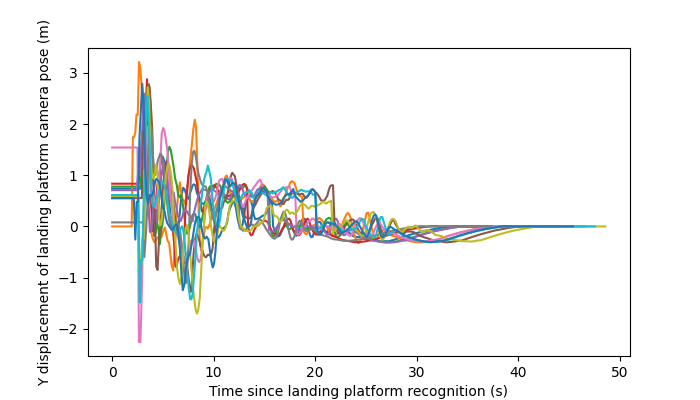
\includegraphics[width=\textwidth]{images/y_displacement.png}
%         \caption{Landing platform Y displacement in camera frame.}
%         \label{subfig:y_displacement}
%     \end{subfigure}
%     \caption{Time versus linear displacement in X and Y directions for landing platform pose in camera frame.}
%     \label{subfig:gimbal_x_y_displacement}
% \end{figure}

The pose of the landing platform in the $z$ direction behaves differently, in that it converges to some non-zero distance representing the depth of the landing platform in the camera frame. As the drone approaches the landing platform, this depth of course decreases to near-zero as the drone lands.

\begin{figure}[ht]
    \centering
    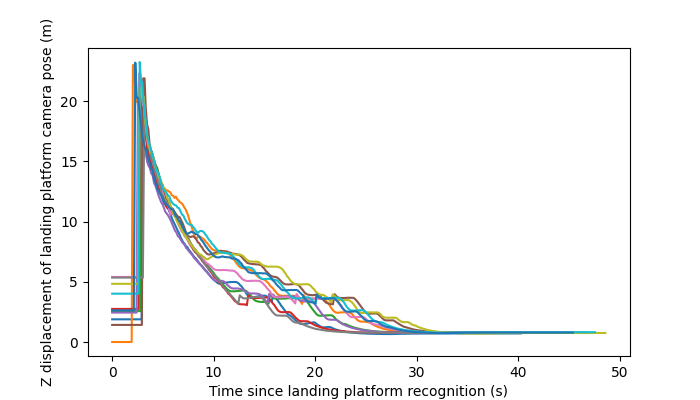
\includegraphics[width=0.7\textwidth]{images/z_displacement.png}
    \caption[Landing platform $z$ displacement in camera frame versus time.]{Landing platform $z$ displacement in camera frame versus time. Each line represents a single attempt to aim the camera during landing.}
    \label{fig:gimbal_z_displacement}
\end{figure}

\section{WhyCon Pose Estimation}

% \begin{figure}[ht]
%     \centering
%     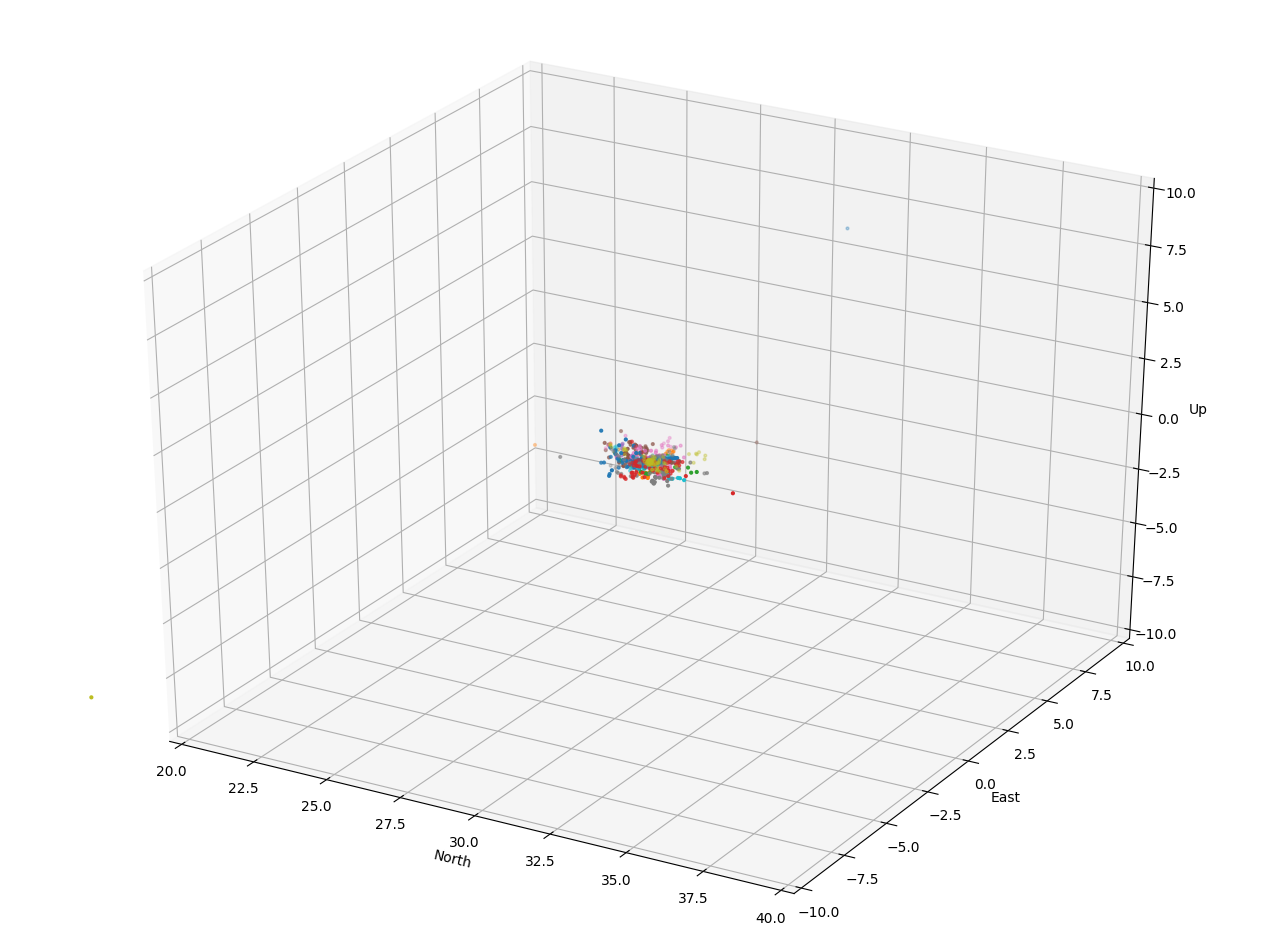
\includegraphics[width=0.9\textwidth]{images/whycon_pose_estimation.png}
%     \caption{WhyCon stationary pose estimation without outliers.}
%     \label{fig:whycon_stationary_pose_estimation}
% \end{figure}

WhyCon markers, as previously known, provide a good means of pose estimation in 3 dimensions, especially in stationary scenarios. Stationary WhyCon pose estimation was therefore the first step in testing the drone's ability to identify the landing platform's position. In configuring the WhyCon system, the outer diameter of the WhyCon marker is a required point of data. The WhyCon module makes it easy to configure this in real time using \texttt{rqt\_reconfigure}. The calibration was quite simple regardless, as the marker was intentionally sized to 1 (simulated) meter in Gazebo. The results of the system calibrated in this way are shown below.

\begin{figure}[ht]
    \centering
    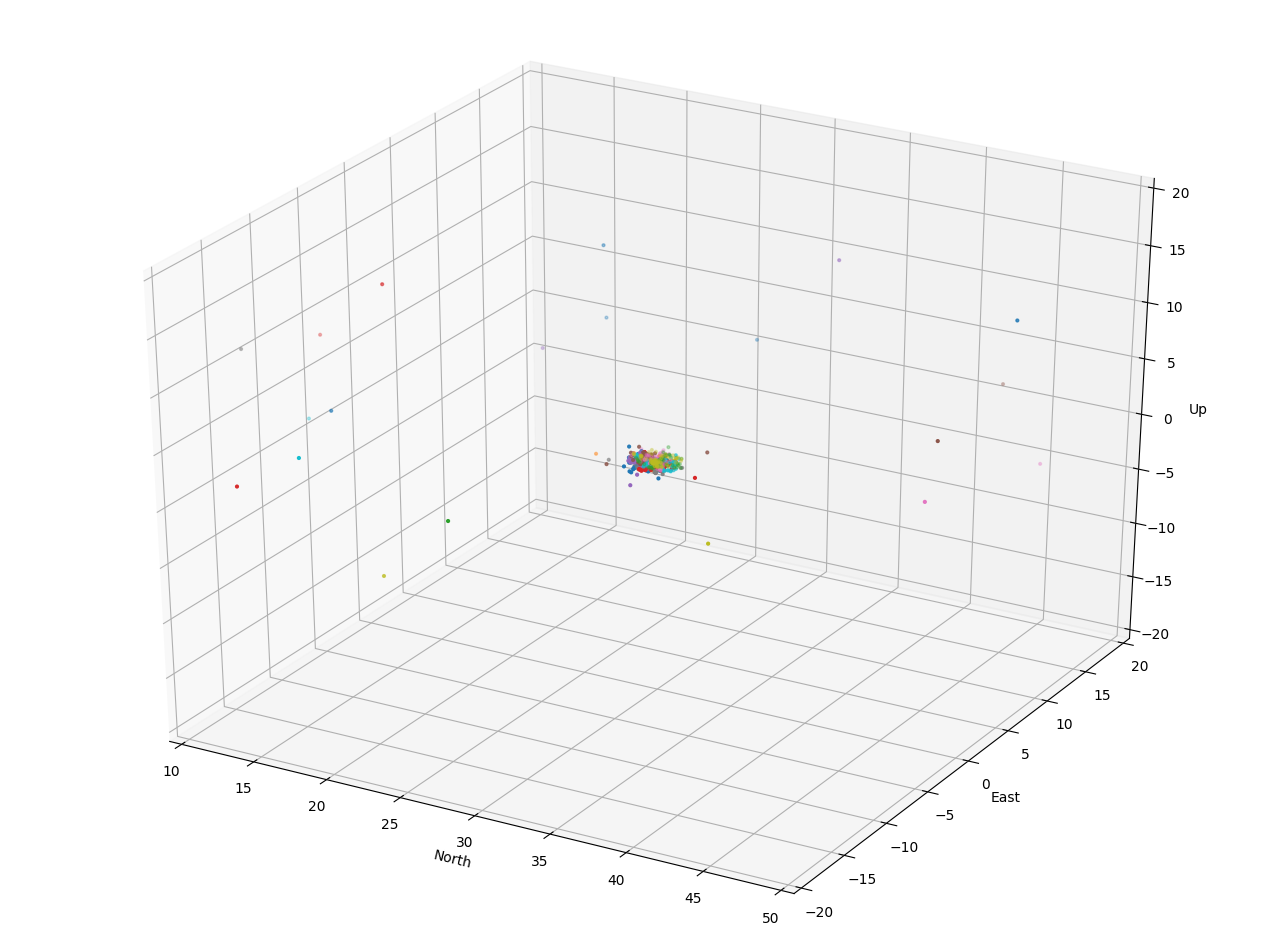
\includegraphics[width=0.85\textwidth]{images/whycon_pose_estimation_with_outliers.png}
    \caption[WhyCon stationary pose estimation with outliers included.]{WhyCon stationary pose estimation with outliers included. This shows that the majority of the poses are concentrated in a small area, and the outliers are relatively few.}
    \label{fig:whycon_stationary_pose_estimation_with_outliers}
\end{figure}

The WhyCon marker is the intended landing site of the drone. In the stationary landing scenario, it was placed at (0, 30, 0) and, as shown in Figure \ref{fig:whycon_stationary_pose_estimation_with_outliers}, the drone is able to reliably estimate the pose of the WhyCon marker. There is transient angular movement in the camera from the moment that the system recognizes the marker to the moment that the camera centers on the marker, which cannot practically be avoided except in truly theoretical scenarios. Moreover, this transient state provides noise which the system must overcome in a real scenario, so neglecting it does no good. Table \ref{tab:stationary_whycon_pose_estimation} outlines the average pose estimations in each dimension ($\mu_x, \mu_y, \mu_z$), as well as the standard deviations in each dimension ($\sigma_x, \sigma_y, \sigma_z$). The average estimations of the landing pad's position in the plane are roughly accurate, $\mu_x = 0.008 \approx 0$ and $\mu_y = 29.704 \approx 30$. Their standard deviations of $\sigma_x=0.996$ and $\sigma_y=0.518$ are acceptable and expected levels of variation. The pose estimate in the $z$ axis is somewhat harder to estimate conceptually - especially with a monocular camera - and this is reflected in the clear overestimation of the relative distance from the drone to the marker in the z axis. While the true value of the position of the WhyCon marker in the z axis is 0, the average estimate value is $\mu_z=-0.050$, actually putting the marker below the ground! However, an overestimate in the z axis of the WhyCon marker is not prohibitively destructive, as the WhyCon marker is not even used for final descent since it will by then be out of the field of view of the camera.

\begin{table}[ht]
    \centering
    \begin{tabular}{|c|r|}
    \hline
        $\mu_x$ &  0.008\\\hline
        $\mu_y$ &  29.704\\\hline
        $\mu_z$ &  -0.050\\\hline
        $\sigma_x$ &  0.996\\\hline
        $\sigma_y$ &  0.518\\\hline
        $\sigma_z$ &  0.142\\\hline
        $n$ & 1292\\\hline
    \end{tabular}
    \caption{Means and standard variations for stationary WhyCon estimation.}
    \label{tab:stationary_whycon_pose_estimation}
\end{table}

Figure \ref{fig:whycon_stationary_pose_estimation_with_outliers} shows some of the outliers in the WhyCon pose estimation. It is worth mentioning that these outliers exist, although they do not drastically affect the pose estimation. One mitigating factor that negates the effect of these outliers is that the WhyCon ``callback'' function estimates the pose of the landing pad at roughly 30 Hz, such that the 17 outliers represent just slightly more than 0.5 seconds of actual runtime, and the rest of the estimates are much closer to the correct value. Further, as differently colored dots represent different samplings, each outlier represents only a minuscule amount of inaccurate pose estimation time per approach. These outliers seem to be caused by the initially inaccurate pose estimation of the marker upon its first detection in a moving frame.

% \begin{figure}[ht]
%     \centering
%     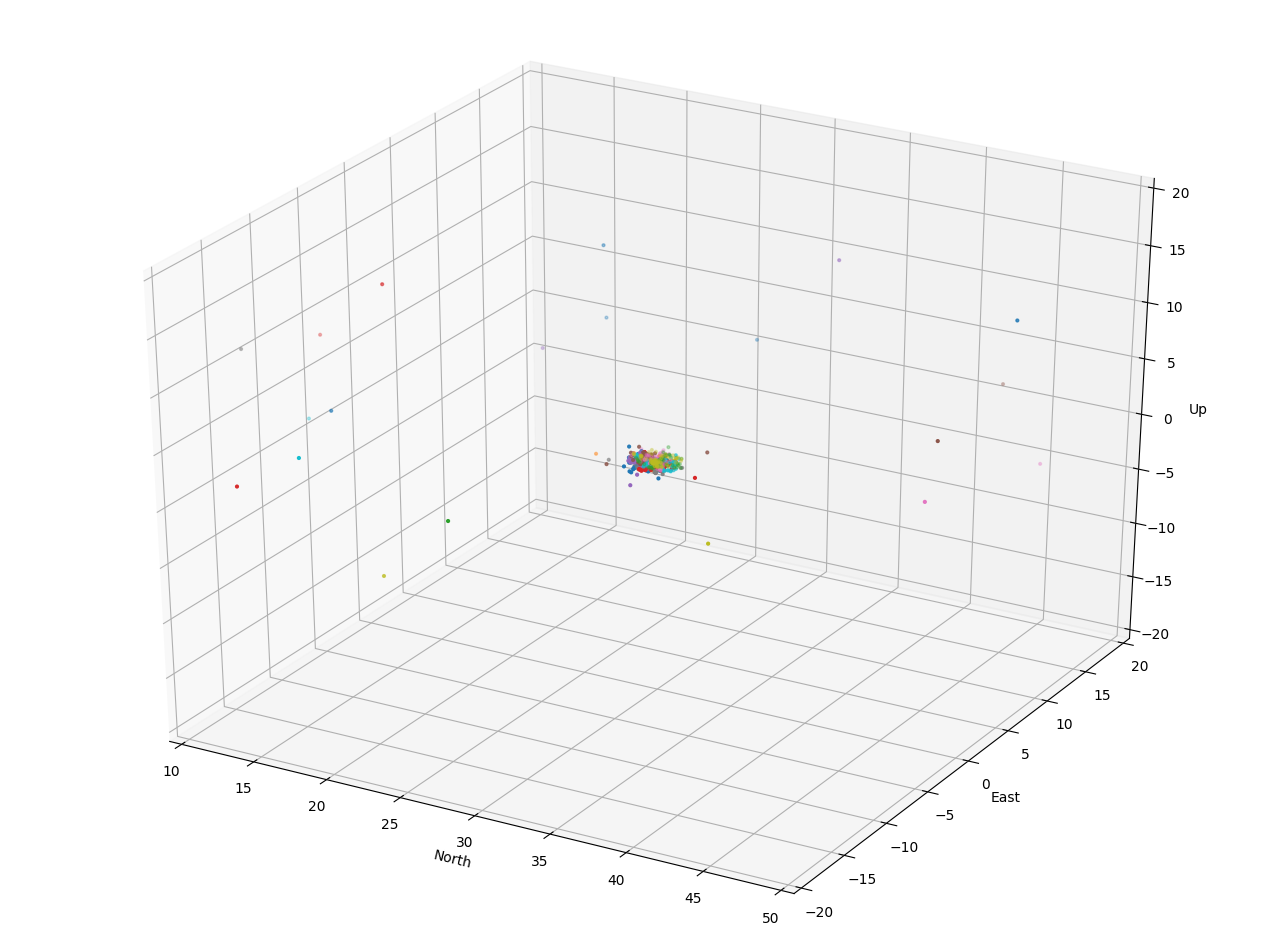
\includegraphics[width=0.9\textwidth]{images/whycon_pose_estimation_with_outliers.png}
%     \caption{WhyCon stationary pose estimation with outliers included.}
%     \label{fig:whycon_stationary_pose_estimation_with_outliers}
% \end{figure}

Figure \ref{fig:whycon_stationary_error} shows a graph of the magnitude of the 3-dimensional WhyCon pose estimate error over the course of 10 approaches. That is, if the error $e$ of the estimate has components $e_x,e_y,e_z$, the plotted value for the magnitude of this error is simply $|e|=\sqrt{e_x^2+e_y^2+e_z^2}$: the Euclidean distance between the true value and estimated value of the position of the WhyCon marker. These results generally show an increase in pose estimation error when the distance from the marker increases. A regression line following Equation \ref{equation:whycon_error_regression} estimates the relationship between the WhyCon pose estimation error and the distance to the WhyCon marker, where $y$ denotes the pose estimation error and $x$ denotes the distance to the marker. The standard error for this regression is $\sigma=0.0154$ over the $n=1292$ samples. The main takeaway from this result is that the WhyCon marker can be used from a distance of about 1 meter to a distance of about 18 meters. When the drone is closer than 1 meter to the landing platform, the WhyCon marker is out of the camera's field of view, and when the drone is sufficiently far away from the landing platform, the marker is simply not recognizable. 

\begin{equation}
    y=-0.004x^3+0.180x^2-0.876x+1.843
    \label{equation:whycon_error_regression}
\end{equation}

\begin{figure}[ht]
    \centering
    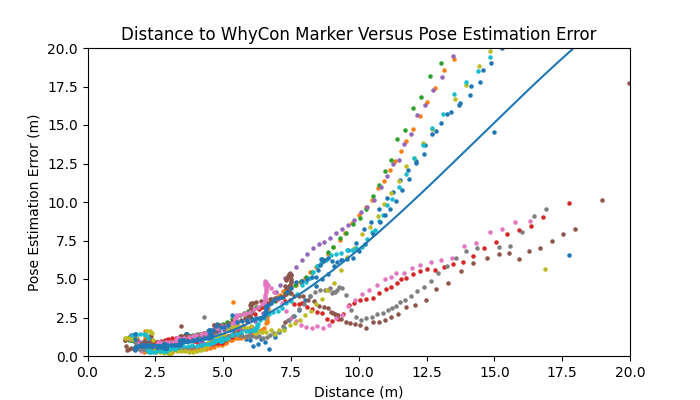
\includegraphics[width=0.65\textwidth]{images/whycon_pose_estimation_error.png}
    \caption{Distance to WhyCon marker vs. magnitude of 3-dimensional pose estimate error.}
    \label{fig:whycon_stationary_error}
\end{figure}



\subsection{WhyCode Trials}
\label{subsection:whycode_trials}

% {\color{red}This section ``WhyCode Trials'' will provide an explanation for the attempt made to use WhyCode and the reasons why it failed in this scenario. WhyCode markers are preferable to WhyCon markers because, in theory, they can provide unambiguous yaw orientation unlike WhyCon markers. However, in each set of WhyCode markers (sets are grouped by the number of bits contained in their IDs), there are necessarily markers that are rotationally equivalent to each other, but with different IDs. The current implementation of \texttt{whycon\_ros} is able to identify the ID of whichever WhyCode marker it sees, but it may determine the ID of a rotationally symmetric marker instead of the intended marker. A workaround for this was attempted: 2-bit WhyCode markers with ID 1 and 2 are rotationally symmetric, but have two distinct sides, so that if ID 1 is recognized, then the orientation could theoretically be used without modification, and if ID 2 is recognized, then the orientation could be flipped by $\pi$ radians in the axis normal to the marker. The GUI even unambiguously identifies the yaw of the marker, but the orientation of the marker in the published ROS topic changes unpredictably (by $\pi$ radians in the marker's z-axis, without a change in the marker's recognized ID), which causes non-negligible issues in the pose estimation. This route is still worth pursuing because of the simpler and more robust algorithm used in recognizing WhyCon/WhyCode markers. A WhyCode marker could replace the AprilTag marker that is used for final descent.}

The original landing platform design was a single WhyCode marker. This minimalistic design could simplify the system by lessening the amount of coordinate system transforms and components within the gimbal controller, as well as the physical landing platform itself. However, due to two issues, this option was abandoned in favor of the aforementioned landing platform design.

The first issue is that each set of WhyCode markers (where a group is defined by the number of bits contained in the group's IDs) contains rotationally symmetric markers. This is true for markers with more than a single ID bit. This is shown in Figure \ref{fig:whycode_rotational_symmetry}, where the number of ID bits is 2. Moreover, markers such as those with IDs 3 and 4 do not provide an unambiguous orientation, as there is no way to define a unique ``front'' on the marker. However, the markers with IDs 1 and 2, though rotationally equivalent to each other, do have a potential ``front'' which would allow for the unambiguous determination of the marker's yaw. The original plan for the system design involved placing the ``front'' of the marker at the center of the larger white semi-circle of a WhyCode marker with ID 1. The anticipated workaround for the problem of the marker's rotational symmetry was to use the natural orientation of the marker if the \texttt{whycon\_ros} system recognized its ID as 1, and to apply an initial rotation of $\pi$ radians about the marker's central z axis if it was recognized with an ID of 2. In theory this method should still work, but it was never fully attempted because of the second issue.

\begin{figure}[ht]
    \begin{subfigure}[b]{0.23\textwidth}
        \centering
        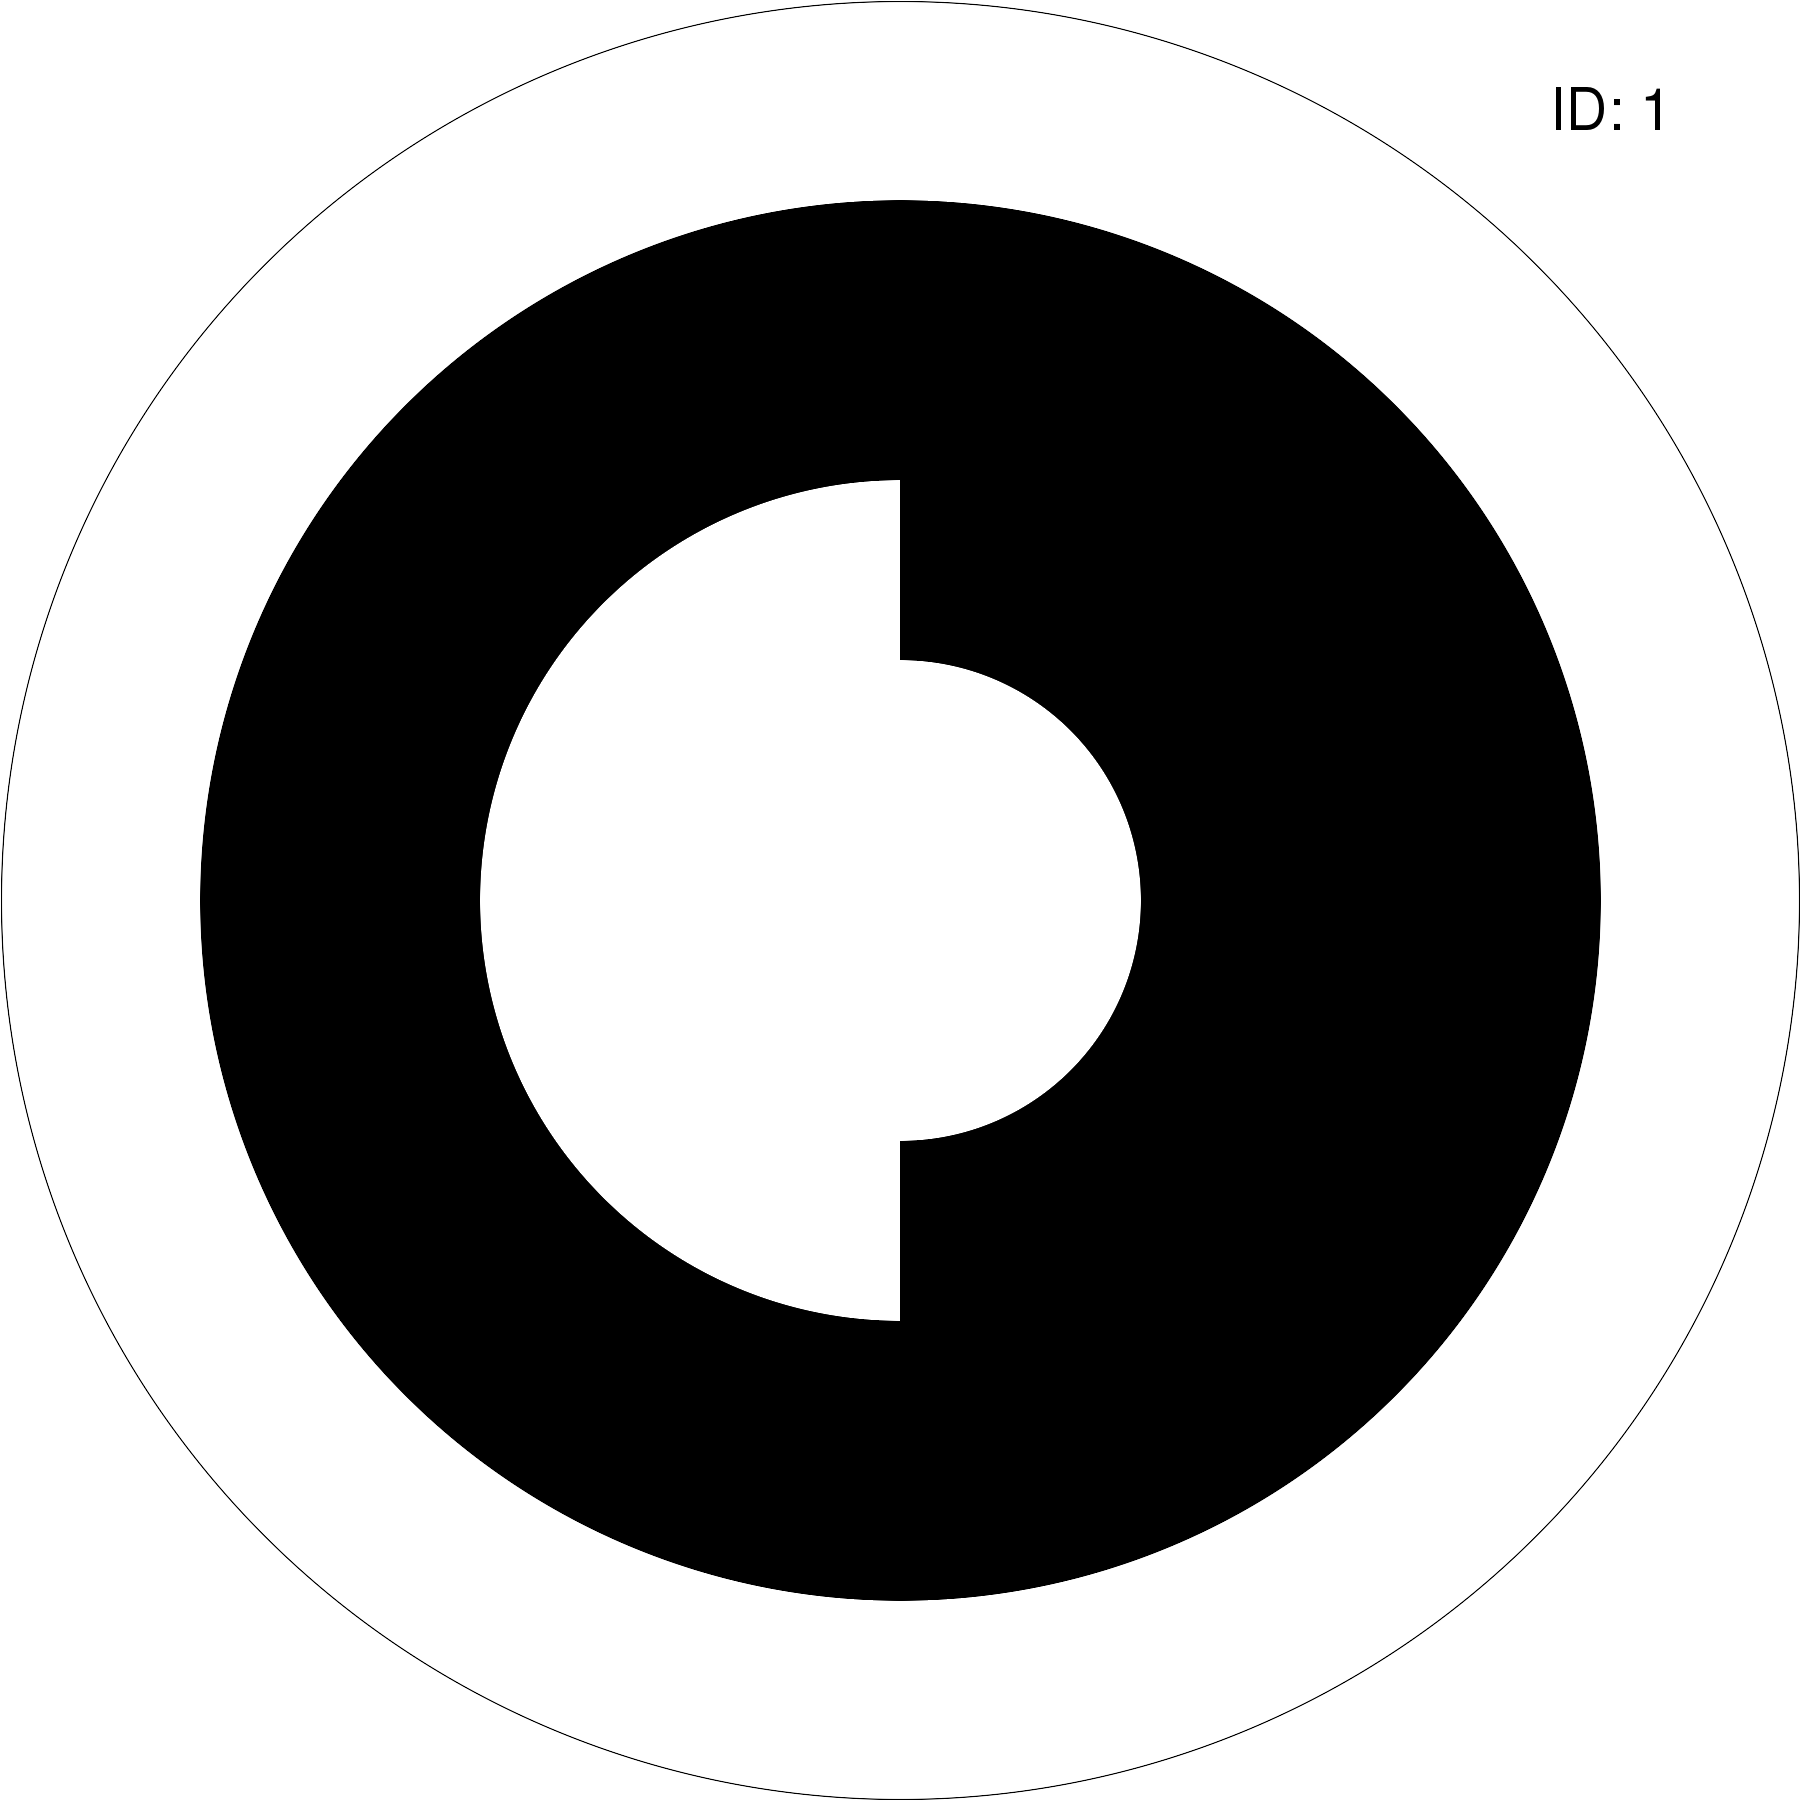
\includegraphics[width=\textwidth]{images/00000001.png}
        % \caption{``Chessboard'' detection.}
        \label{subfig:whycode_1}
    \end{subfigure}
    \begin{subfigure}[b]{0.23\textwidth}
        \centering
        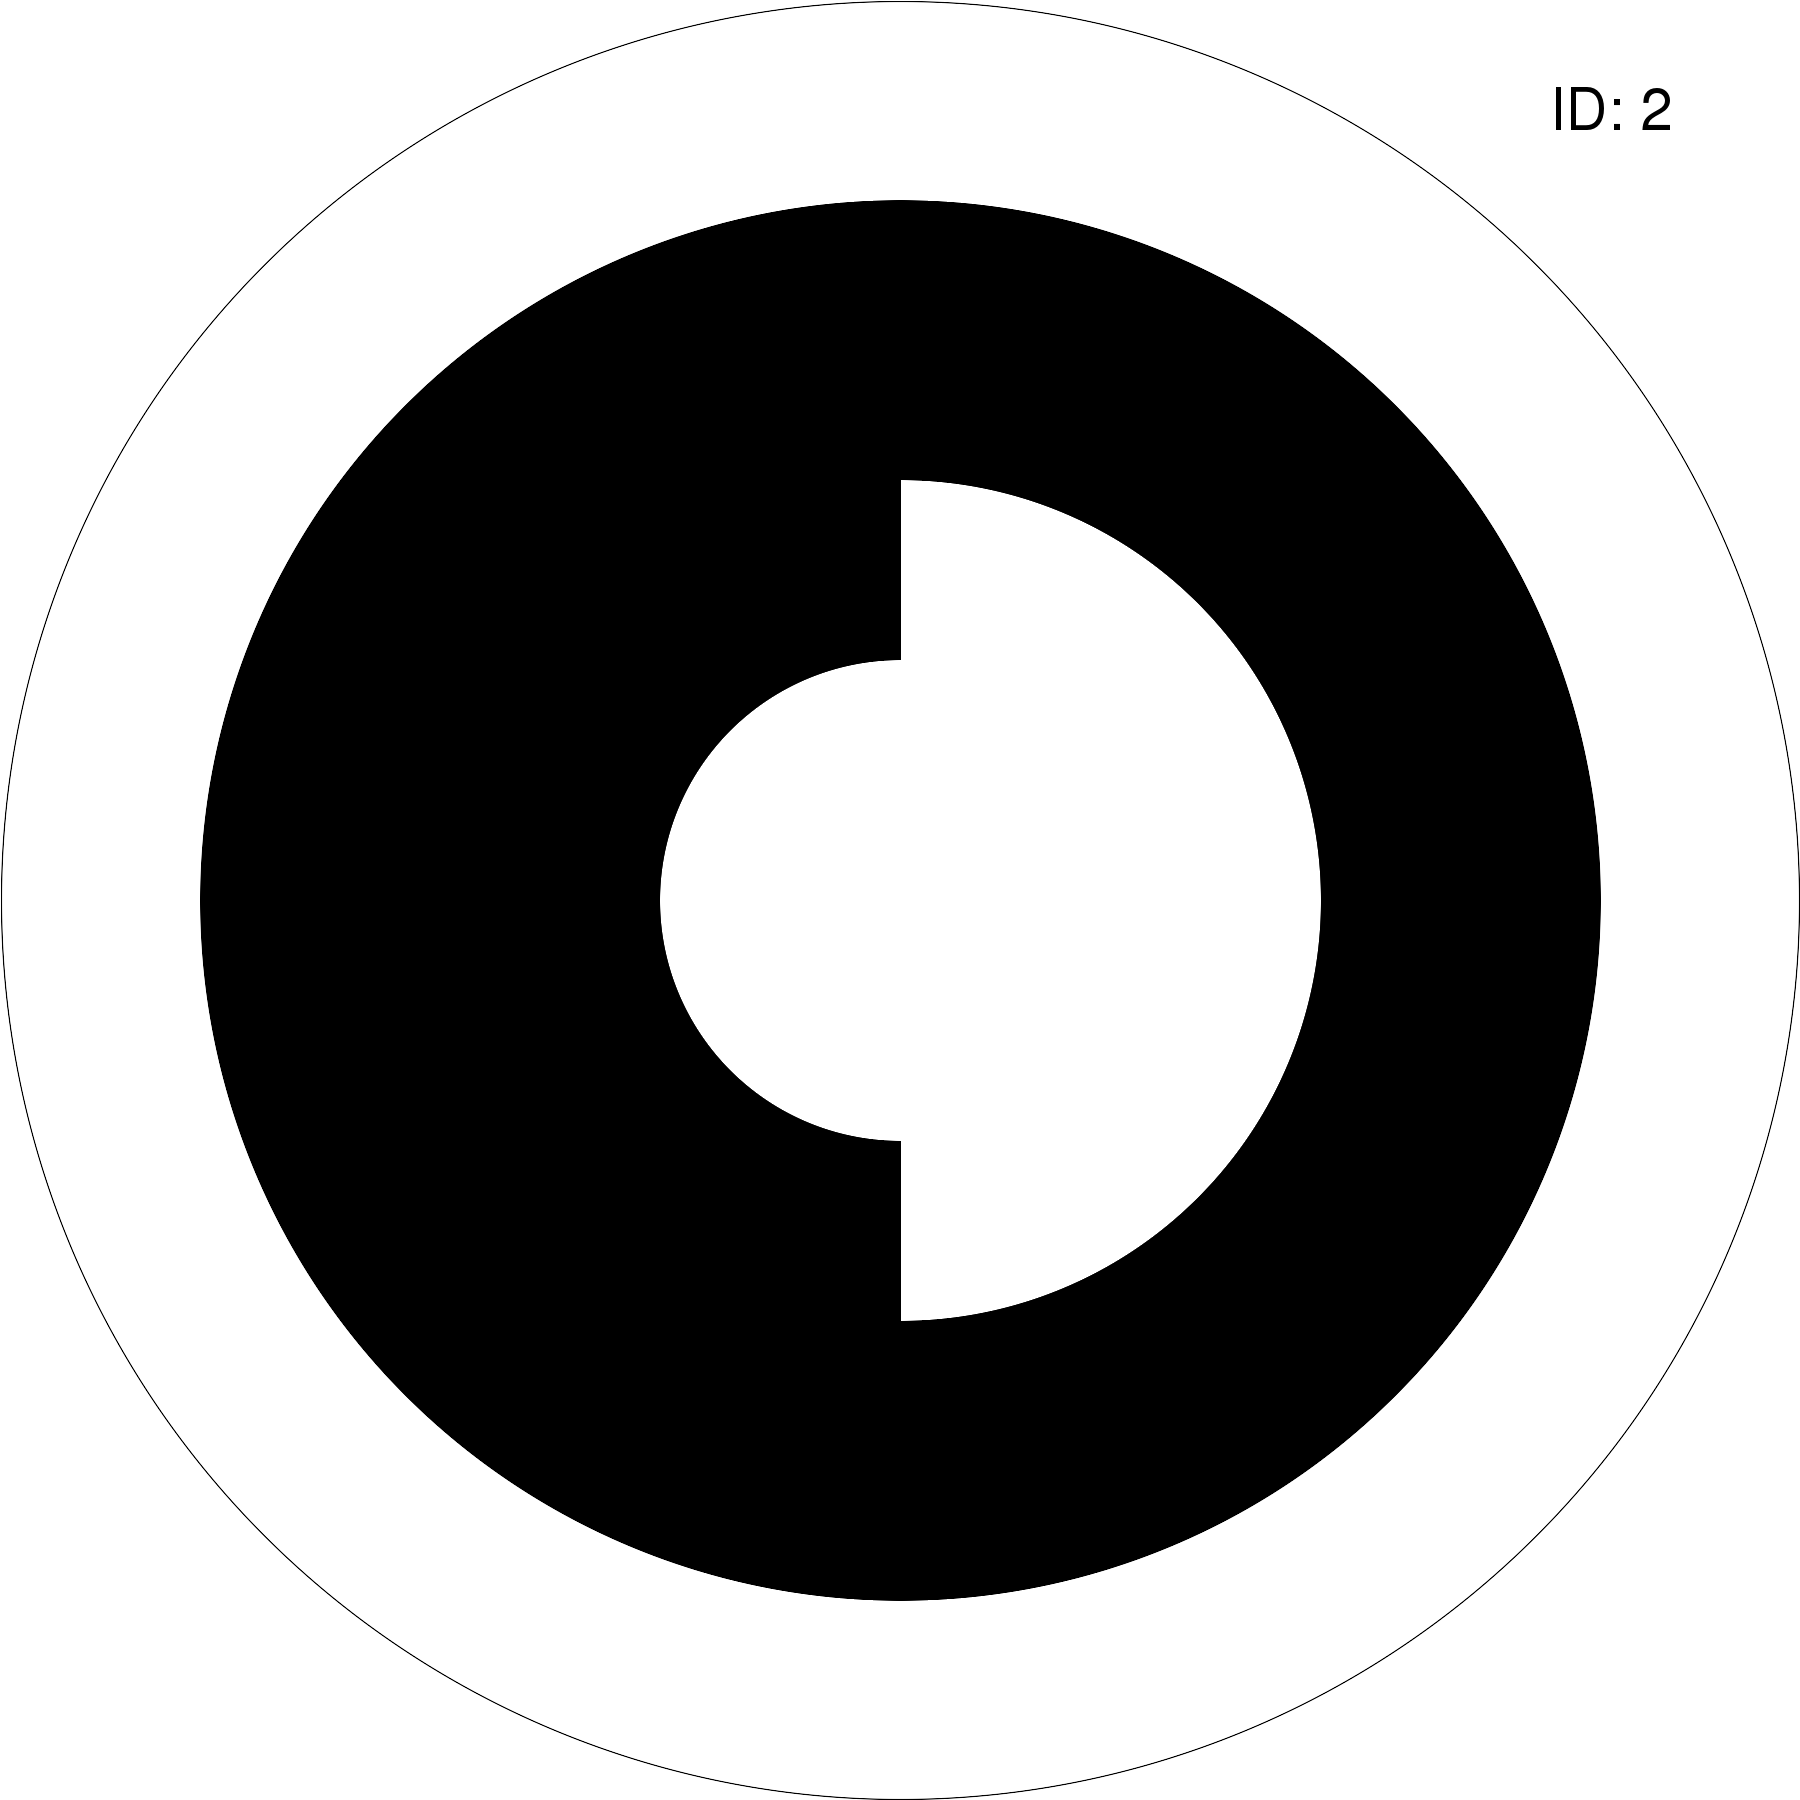
\includegraphics[width=\textwidth]{images/00000002.png}
        % \caption{``Chessboard'' detection.}
        \label{subfig:whycode_2}
    \end{subfigure}
    \begin{subfigure}[b]{0.23\textwidth}
        \centering
        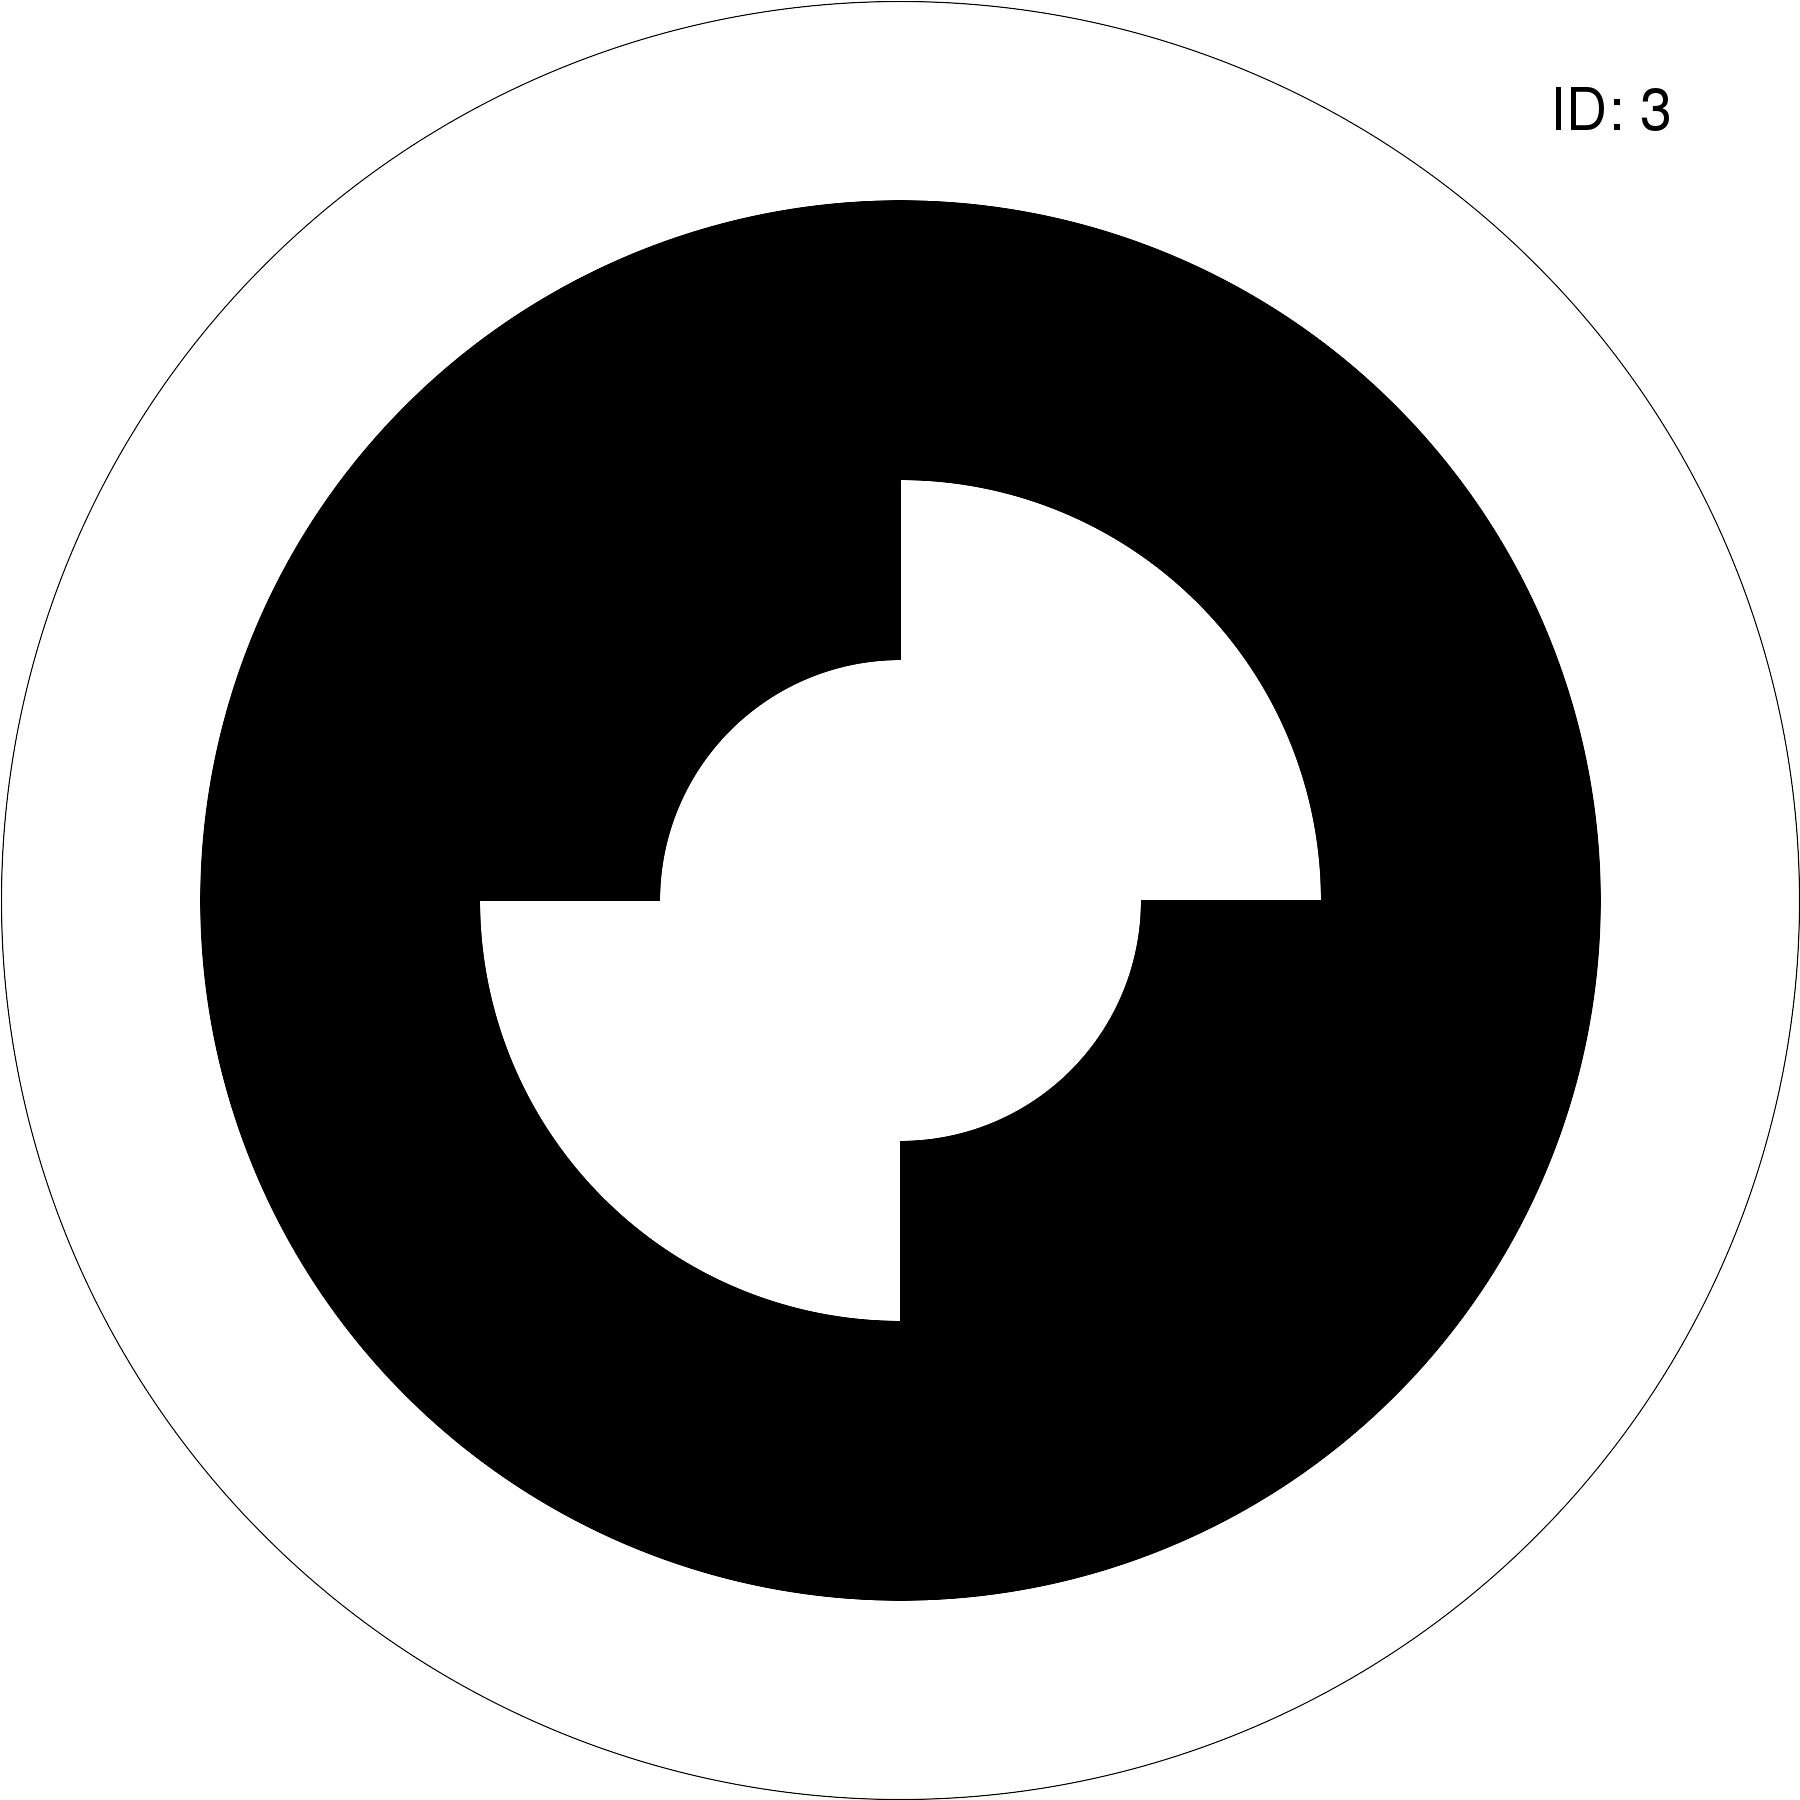
\includegraphics[width=\textwidth]{images/00000003.png}
        % \caption{``Chessboard'' detection.}
        \label{subfig:whycode_3}
    \end{subfigure}
    \begin{subfigure}[b]{0.23\textwidth}
        \centering
        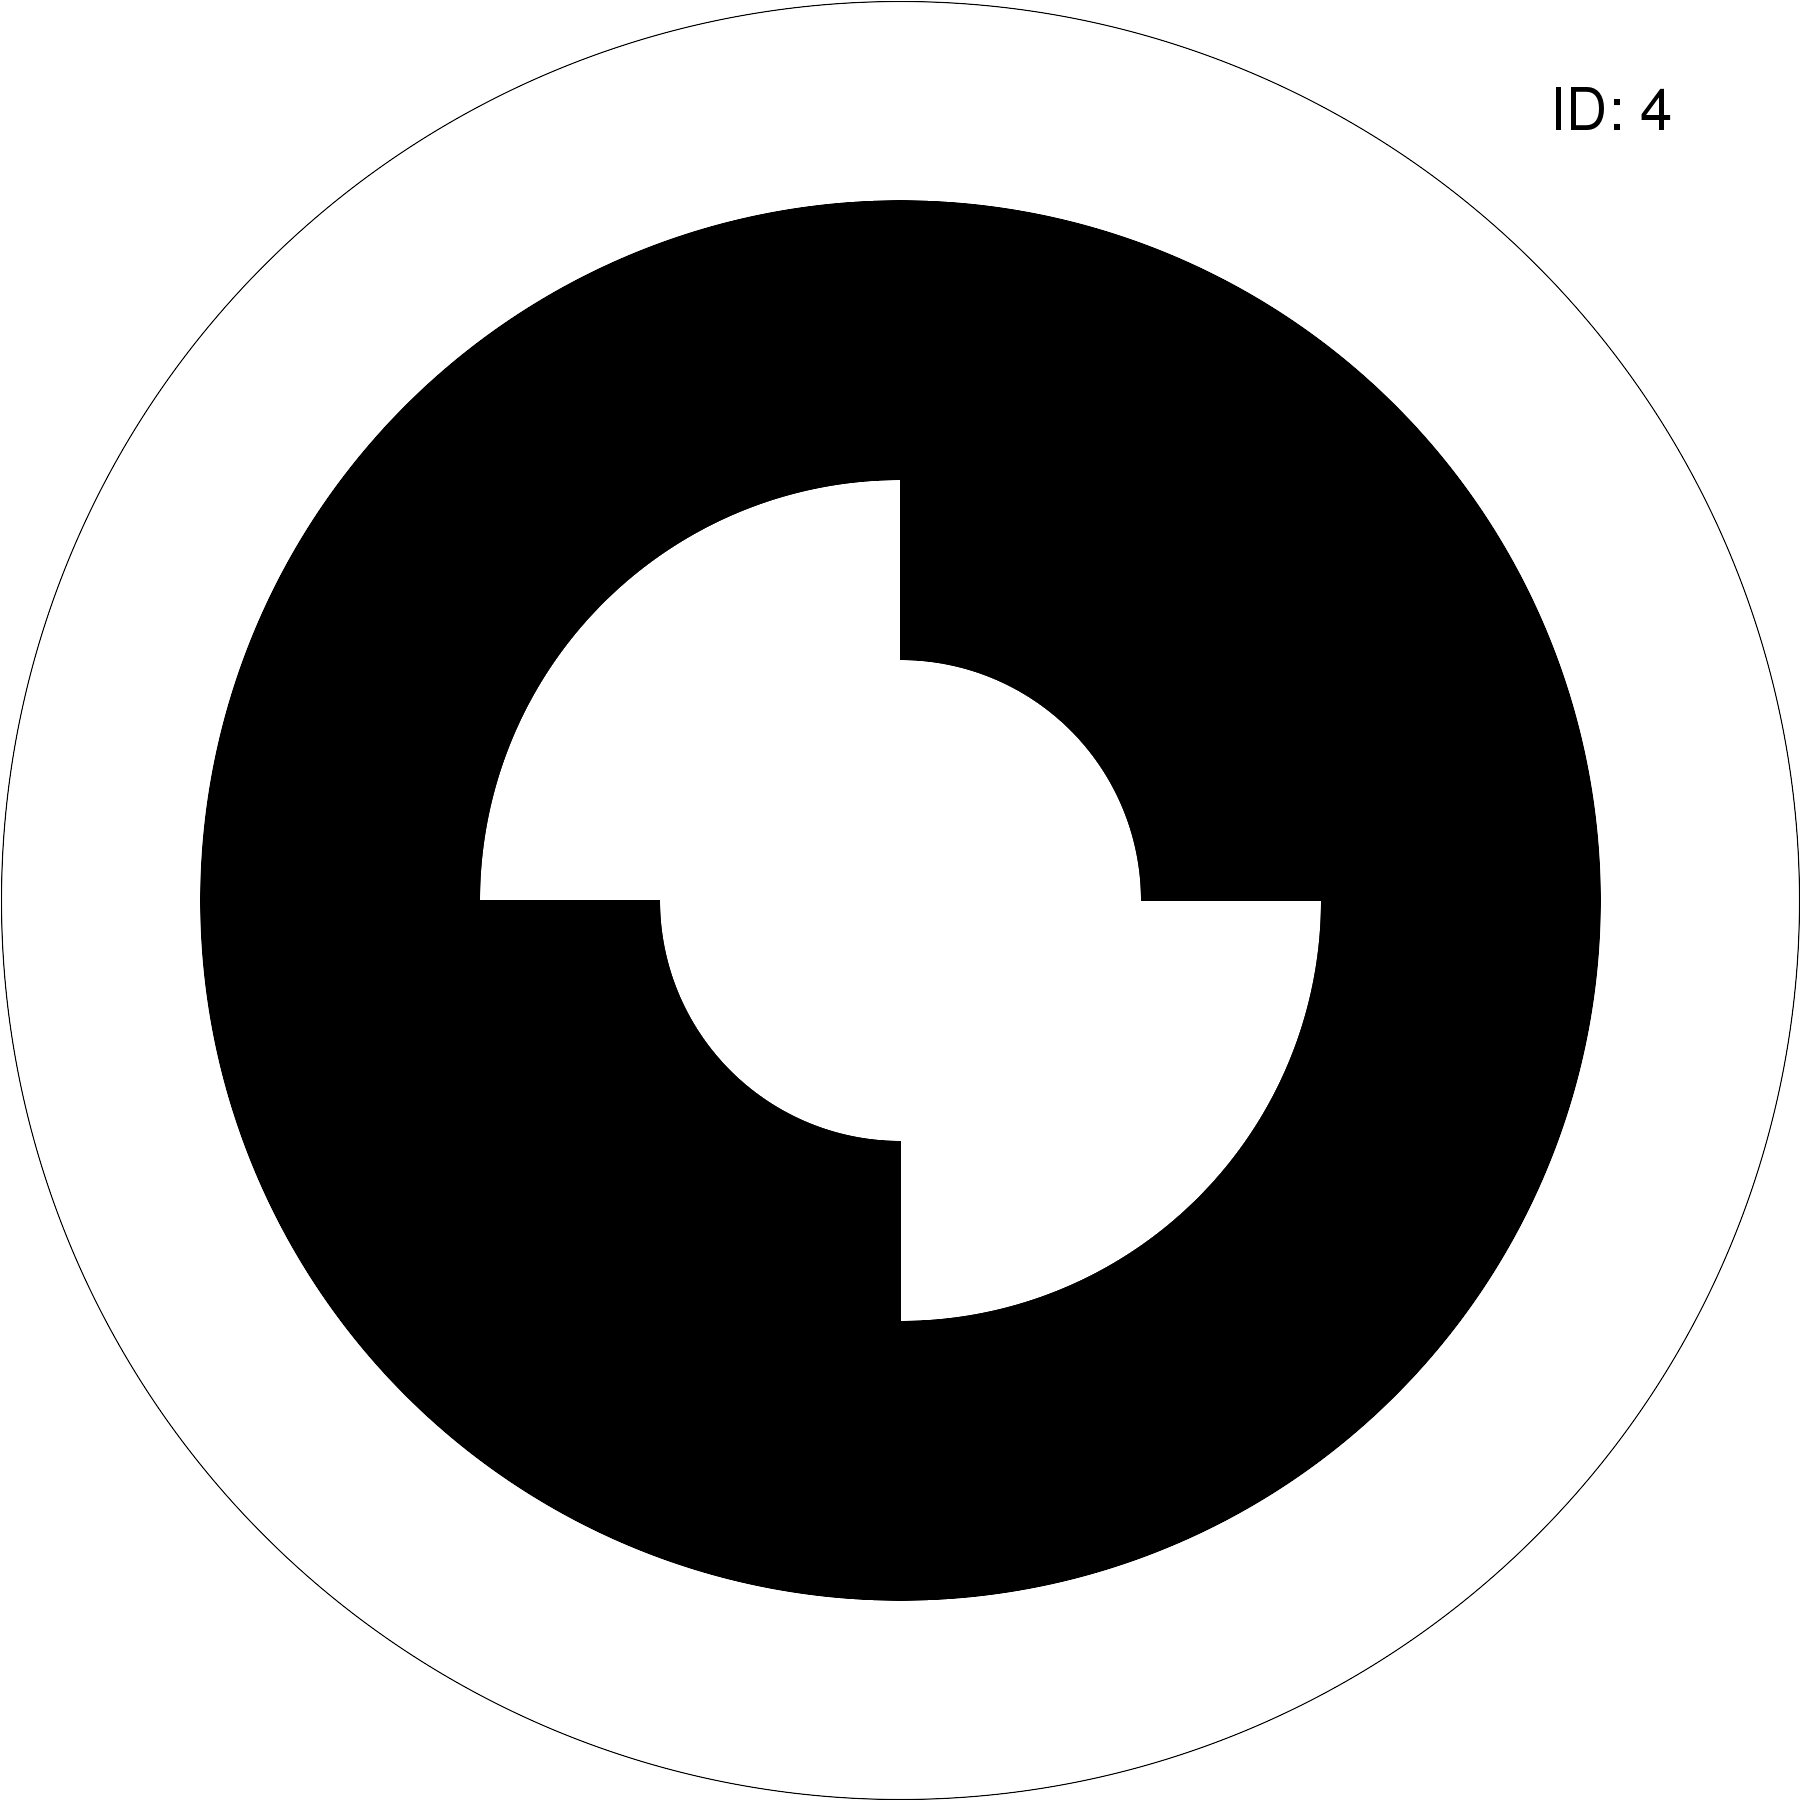
\includegraphics[width=\textwidth]{images/00000004.png}
        % \caption{``Chessboard'' detection.}
        \label{subfig:whycode_4}
    \end{subfigure}
    \caption{Rotationally symmetric WhyCode markers with 2 ID bits, generated from the LCAS \texttt{whycode\_id\_gen}.}
    \label{fig:whycode_rotational_symmetry}
\end{figure}

The second issue with using WhyCode markers came from the unanticipated, destructive interaction between the PID systems used to aim the camera, and the WhyCode system. The exact cause of the issue has not been determined, but it corresponds to sign changes in the positional components of the WhyCode marker's pose. This issue only happens specifically when the marker is being identified, and it does not happen every time the marker is identified. This made the issue very hard to isolate. Further investigation into this issue is necessary.

The issue can be illustrated through an experiment, the results of which are shown in Figures \ref{subfig:whycode_camera_position} and \ref{subfig:whycode_camera_orientation}, where the drone was stationary on the ground, viewing a marker in front of it, with the gimbal controller aiming the camera at the marker. As shown in Figure \ref{subfig:whycode_camera_position}, the x and y components of the marker within the camera frame are close to 0, but oscillate, after the marker is detected. This oscillation is to be expected because of the nature of PID controllers, and it is not inherently a problem in itself. However, the orientation of the marker is an important component of the pose, and, as Figure \ref{subfig:whycode_camera_orientation} shows, the small, acceptable oscillation in the positional components corresponds to large, unacceptable oscillation in the marker's recognized orientation. The oscillation in the orientation does not represent noise, but rather an axial flip without a change in the perceived marker ID. The ultimate result of this was that the marker's pose could not be reliably determined while the WhyCon module's identification functionality was running. Because of this issue, the identified WhyCode markers were temporarily abandoned in favor of the April Tag markers for the determination of the landing platform's yaw.

\begin{figure}
    \centering
        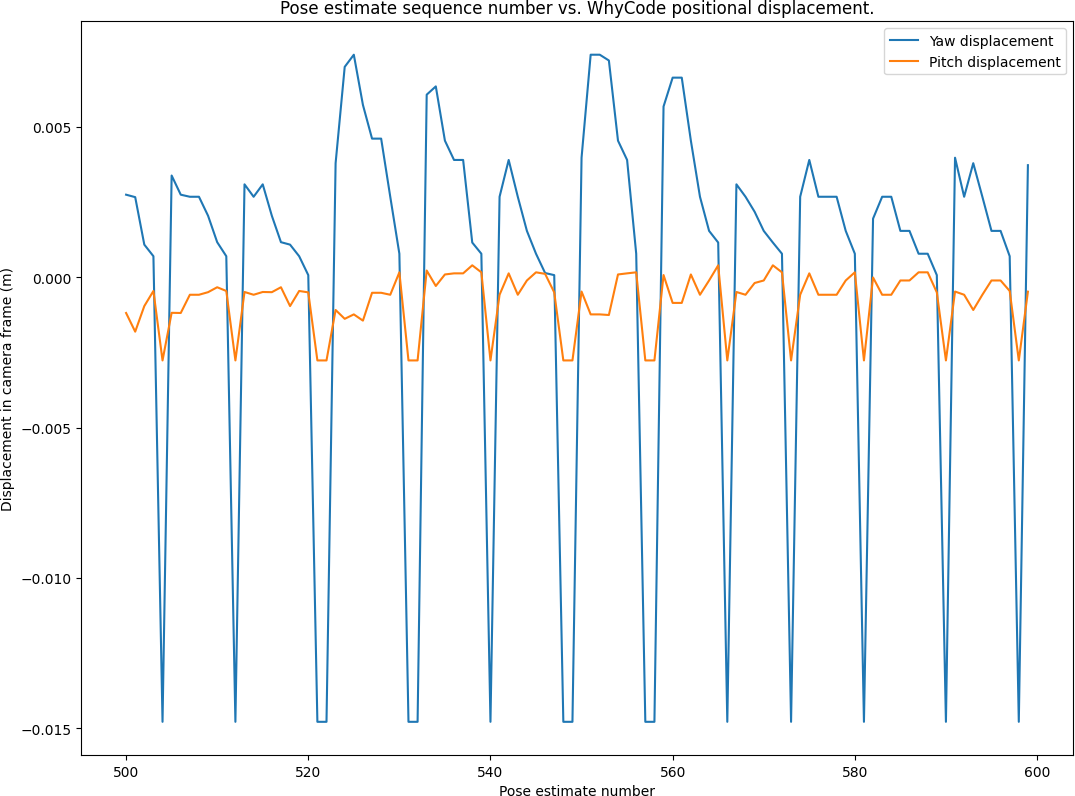
\includegraphics[width=0.8\textwidth]{images/whycode_camera_pose_constrained.png}
        \caption{$x$ and $y$ position components of the WhyCode marker's pose in the camera frame.}
        \label{subfig:whycode_camera_position}
\end{figure}

\begin{figure}
    \centering
        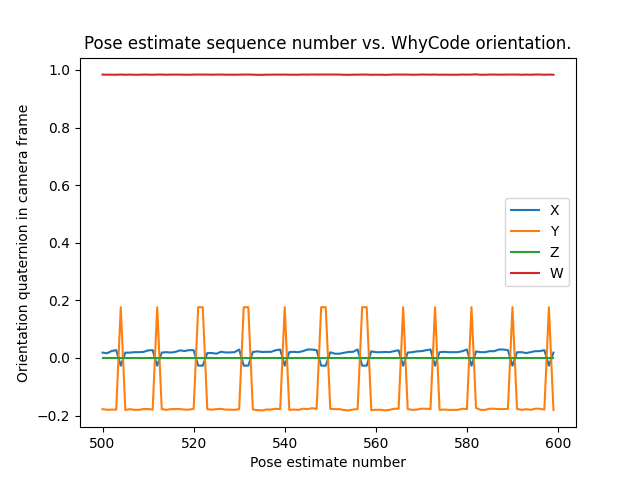
\includegraphics[width=0.7\textwidth]{images/whycode_camera_orientation_constrained.png}
        \caption{$x,y,z,w$ orientation components of the WhyCode marker's pose in the camera frame.}
        \label{subfig:whycode_camera_orientation}
\end{figure}

% \begin{figure}[ht]
%     \centering
%     \begin{subfigure}[b]{0.47\textwidth}
%         \centering
%         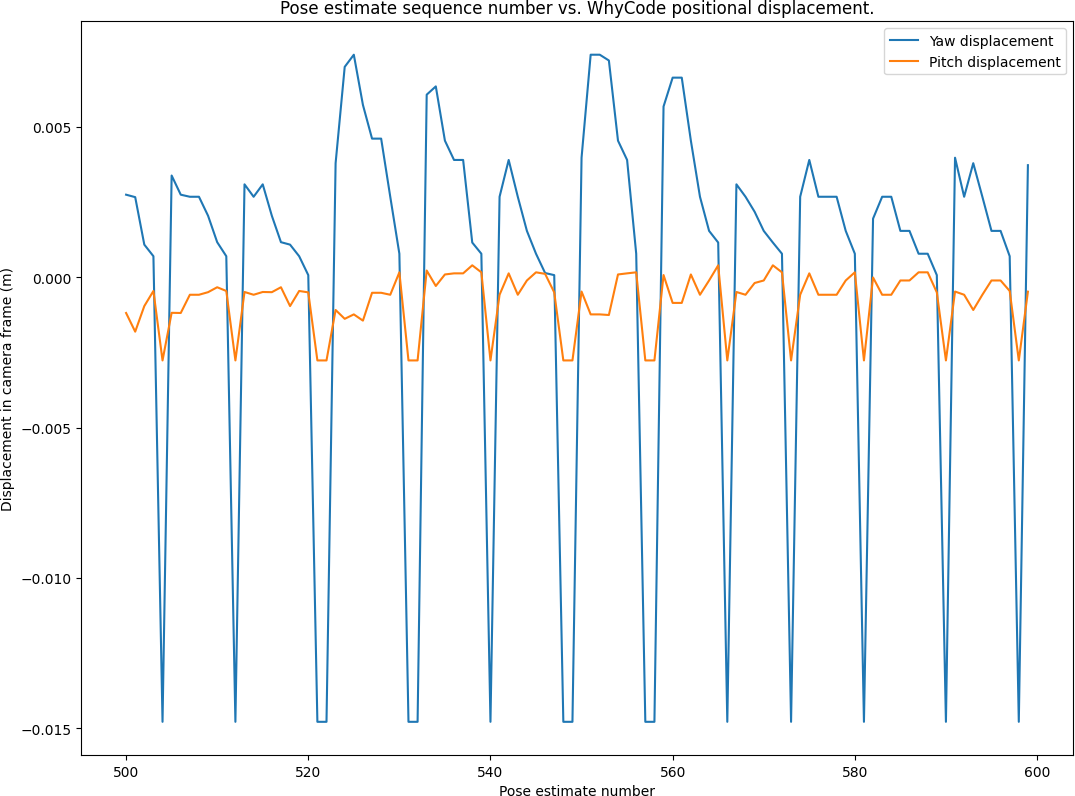
\includegraphics[width=\textwidth]{images/whycode_camera_pose_constrained.png}
%         \caption{$x$ and $y$ position components of the WhyCode marker's pose in the camera frame.}
%         \label{subfig:whycode_camera_position}
%     \end{subfigure}
%     \begin{subfigure}[b]{0.47\textwidth}
%         \centering
%         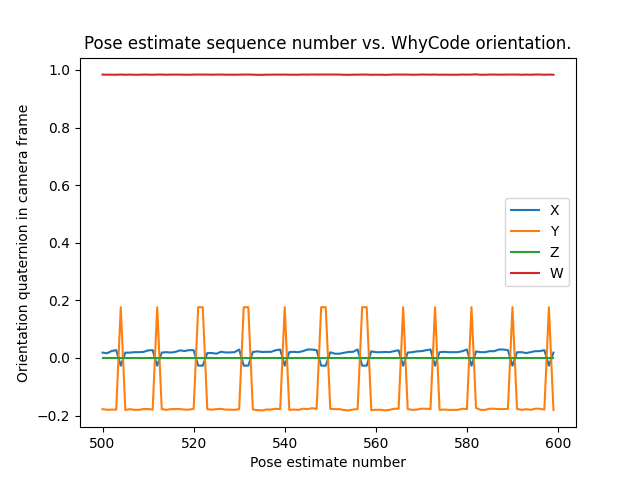
\includegraphics[width=\textwidth]{images/whycode_camera_orientation_constrained.png}
%         \caption{$x,y,z,w$ orientation components of the WhyCode marker's pose in the camera frame.}
%         \label{subfig:whycode_camera_orientation}
%     \end{subfigure}
%     \caption[Destructive interaction between WhyCode system and gimbal controller.]{Destructive interaction between the WhyCode system and gimbal PID controllers, resulting from \gls{PID} oscillation.}
%     \label{subfig:whycode_problems}
% \end{figure}

\begin{figure}[h!]
    \centering
    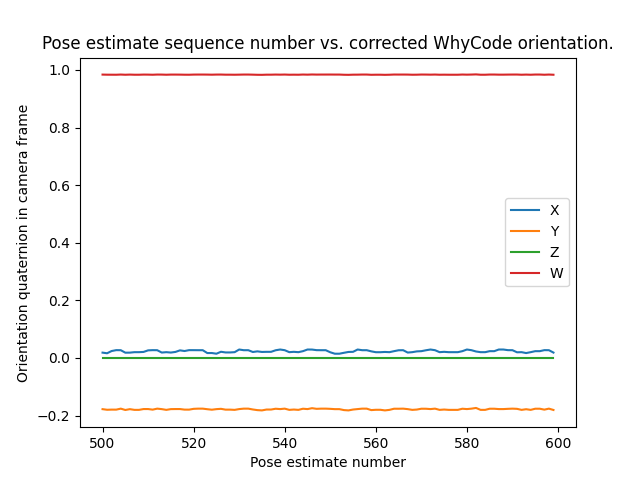
\includegraphics[width=0.5\textwidth]{images/whycode_camera_orientation_constrained_corrected.png}
    \caption[WhyCode marker orientation components after ``fixing.'']{WhyCode marker orientation components after ``fixing.'' This shows that the persistent flipping shown in Figure \ref{subfig:whycode_camera_orientation} has been removed, and the perceived orientation of the WhyCode marker is stable.}
    \label{fig:whycode_problems_corrected}
\end{figure}

A simple, ``bandaid'' method for dealing with the WhyCode orientation problem shown in Figures \ref{subfig:whycode_camera_orientation} and \ref{subfig:whycode_camera_position} has been implemented. Let $i$ represent the index of a detection, and let be a quaternion (Explained in Section \ref{subsection:quaternions}) representing $d_i$ representing the $i\mathrm{th}$ detected orientation. At detection $i$, the gimbal controller stores the orientation, $d_i$, of the marker. It compares the \textit{inverse} of the detected orientation at frame $i+1$, $d_{i+1}^{-1}$ to the orientation of the marker at detection $i+1$. If the angle represented by $d_{i+1}^{-1}$ is within some small angular displacement $\theta_d$ from the angle represented by $d_i$, then the inverse is assumed to be the correct orientation, is used for further calculation, and is stored for comparison at detection $i+2$. Figure \ref{fig:whycode_problems_corrected} shows how this method maintains continuity within the same test shown in Figure \ref{subfig:whycode_camera_orientation}, when $\theta_d=2\degree$. It is somewhat difficult to identify the cause of this error within the WhyCode source, so as a proof of concept, this ``bandaid'' method was used to correct the issue in this particular scenario. While the fix corrects the orientation of the marker in this particular scenario, it did not solve the issue in testing generally.

\section{April Tag Pose Estimation}

Similar experiments to those used to test WhyCon pose estimation were carried out for the April Tag markers. Figure \ref{fig:apriltag_pose_estimation} shows the wide spread of high-error pose estimation for the April Tag over the course of 10 approaches. It is not surprising that the marker of size 0.3125 meters by 0.3125 meters is not accurately located from the same distance as the WhyCon marker. However, since the April Tag marker is only to be used in late descent, this can be overlooked in favor of the marker's performance at lower altitudes. Table \ref{tab:stationary_apriltag_pose_estimation} outlines the performance of April Tag pose estimation during 10 approaches at altitudes between 0 and 10 meters. The standard deviations of the measurements decrease as distance from the marker decreases, while the means remain in the same acceptable region. Similarly to WhyCon, the z component of the April Tag's pose is somewhat incorrectly estimated - but not prohibitively so. 

\begin{figure}[ht]
    \centering
    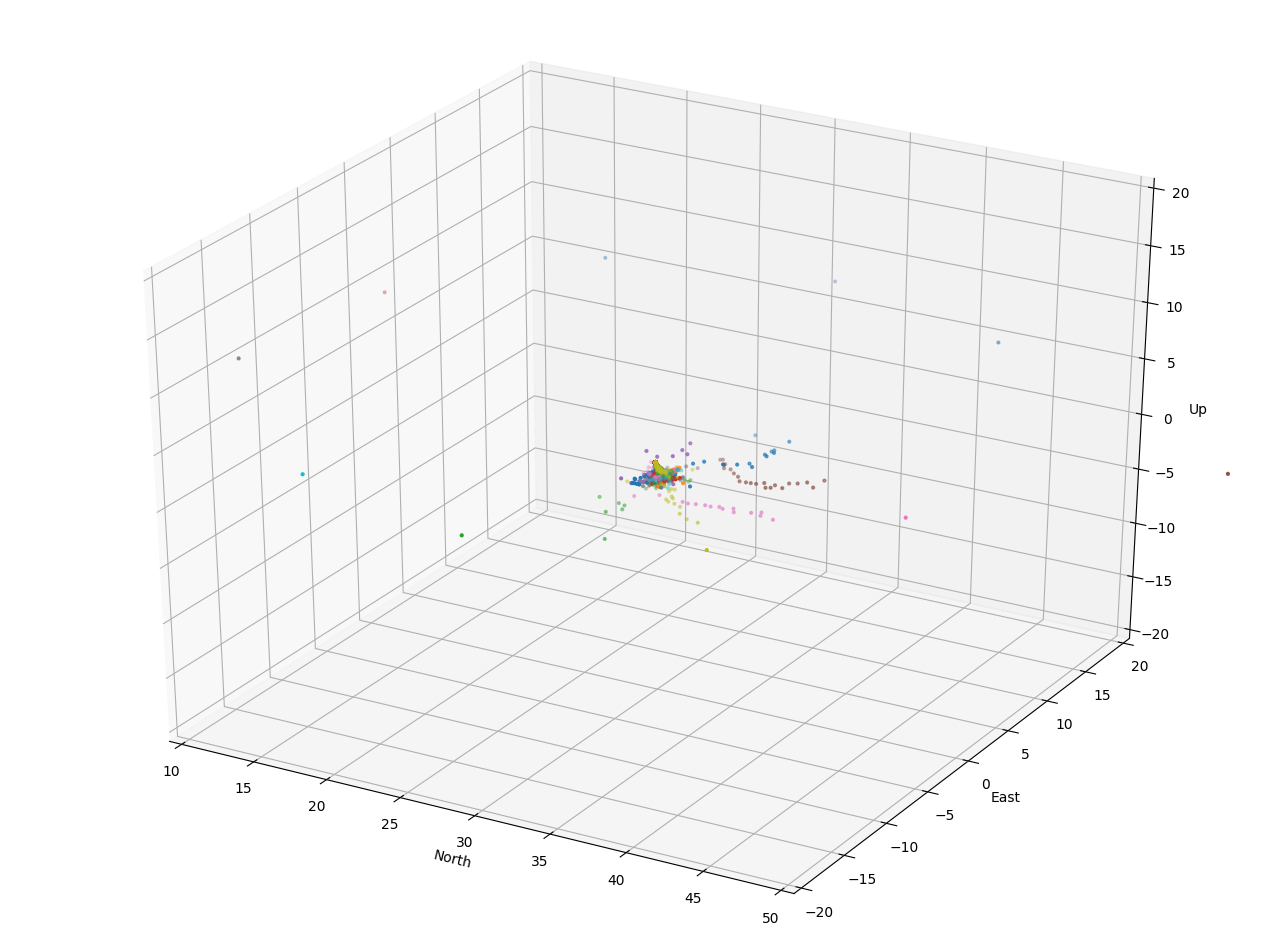
\includegraphics[width=0.85\textwidth]{images/apriltag_pose_estimation.png}
    \caption{April Tag pose estimation.}
    \label{fig:apriltag_pose_estimation}
\end{figure}

\begin{table}[h]
    \centering
    \begin{tabular}{|c|r|}
    \hline
        $\mu_x$ &       0.0720\\\hline
        $\mu_y$ &       30.060\\\hline
        $\mu_z$ &       -0.394\\\hline
        $\sigma_x$ &    1.230\\\hline
        $\sigma_y$ &    1.297\\\hline
        $\sigma_z$ &    0.589\\\hline
        $n$ & 2707\\\hline
    \end{tabular}
    \caption{Means and standard variations for April Tag estimation.}
    \label{tab:stationary_apriltag_pose_estimation}
\end{table}

The pose estimation is visualized in Figure \ref{fig:apriltag_pose_estimation}. The pose was estimated at altitudes varying from 0 to 10 meters in motion, revealing an exponential relationship between the distance from the marker and error in pose estimation magnitude as shown in Figure \ref{fig:apriltag_pose_estimation_error}. The main takeaway from this test is that the error in pose estimation increases with the distance from the marker to the drone, but at close distances the pose estimate is very accurate. Furthermore, the pose estimate is useful to the system throughout the approaches, even in spite of its error. A regression following Equation \ref{equation:april_tag_regression} describes the an estimate of the relationship between the pose estimation error and the distance to the marker, where $y$ denotes the error and $x$ denotes the distance to the marker. The standard error for this regression is $\sigma = 0.0047$ meters over the samples.%, with $n=2707$ samples.

\begin{equation}
    y = -0.002x^3+0.098x^2-0.095x+0.256
    \label{equation:april_tag_regression}
\end{equation}

\begin{figure}[h!]
    \centering
    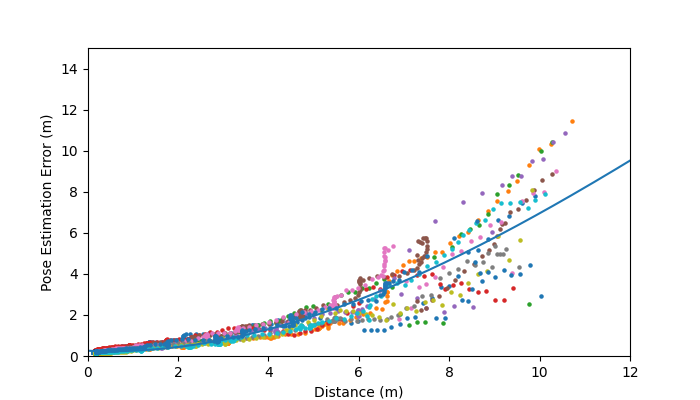
\includegraphics[width=0.65\textwidth]{images/apriltag_pose_estimation_error.png}
    \caption{Pose estimation error versus distance for the April Tag marker.}
    \label{fig:apriltag_pose_estimation_error}
\end{figure}

% The exponential regression generated for this graph shows that the error in pose estimation for the April Tag marker roughly follows the exponential curve described by Equation \ref{equation:apriltag_pose_estimation_error_regression}, where $x$ denotes the Euclidean distance in meters from the drone to the landing platform and $y$ denotes the error in pose estimation in meters. The coefficient of determination is $r^2 = 0.84$, showing that the fit is somewhat loose. This is likely because of the varying and complex motion that the April Tag marker takes in the camera's field of view even during the later portions of approach and landing.

% \begin{equation}
%     y = e^{0.342x - 1.472}
%     \label{equation:apriltag_pose_estimation_error_regression}
% \end{equation}

\subsection{Yaw Estimation}

The yaw of the April Tag is a necessary data point during autonomous landing, as the drone must align itself to the landing pad in order to guarantee that a fiducial marker (in this case, the April Tag) will be in its field of view during the final part of the landing sequence. Thus, the performance of the April Tag's yaw recognition is evaluated. Figure \ref{fig:apriltag_yaw_estimation} shows the perceived yaw angle during the 10 test approaches, and Table \ref{tab:apriltag_yaw_stats} describes them statistically. 


\begin{figure}[h]
    \centering
    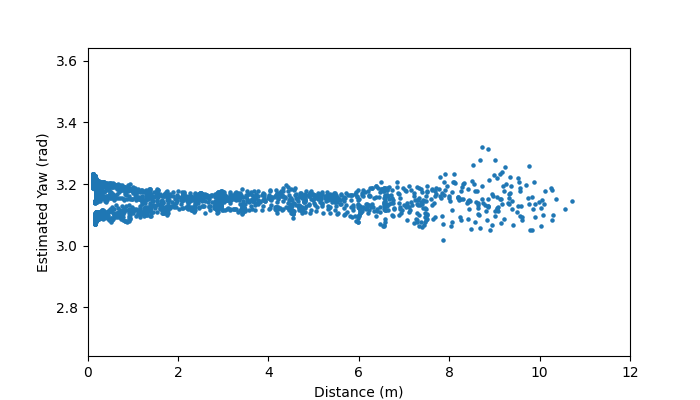
\includegraphics[width=0.65\textwidth]{images/apriltag_yaw_estimation.png}
    \caption{Estimation of the April Tag marker's yaw during the pose estimation approaches.}
    \label{fig:apriltag_yaw_estimation}
\end{figure}

\vspace{-0.25cm}
\begin{table}[ht]
    \centering
    \begin{tabular}{|c|r|}
    \hline
        $\mu_{yaw}$  & 3.149 \\\hline
        $\sigma_{yaw}$ & 0.044 \\\hline
    \end{tabular}
    \caption{}
    \label{tab:apriltag_yaw_stats}
\end{table}

\vspace{-0.25cm}
These show that the yaw estimation of the April Tag marker is quite accurate over its detection range. An angle of $\frac{\pi}{2}$ radians represents due north, however the April Tag marker has been rotated by an additional $\frac{\pi}{2}$ radians in its position on the landing platform, giving the estimated yaw of $3.149 \approx \pi$ radians. Figure \ref{fig:apriltag_yaw_estimation_error} shows the absolute value of the April Tag's yaw estimation error. It is apparent that the yaw estimation error has increases when the distance from the landing platform is both very high and very low. A regression following Equation \ref{equation:apriltag_yaw_error_regression} describes the relationship between the yaw estimation error and the distance to the April Tag marker, with $y$ denoting the yaw estimation error in radians and $x$ denoting the distance to the marker in meters. The standard error of the regression is $\sigma=0.0306$ radians over the $n=2707$ samples.

\begin{equation}
    y=0.003x^2-0.018x+0.051
    \label{equation:apriltag_yaw_error_regression}
\end{equation}

% \vspace{-0.25cm}
\begin{figure}[h!]
    \centering
    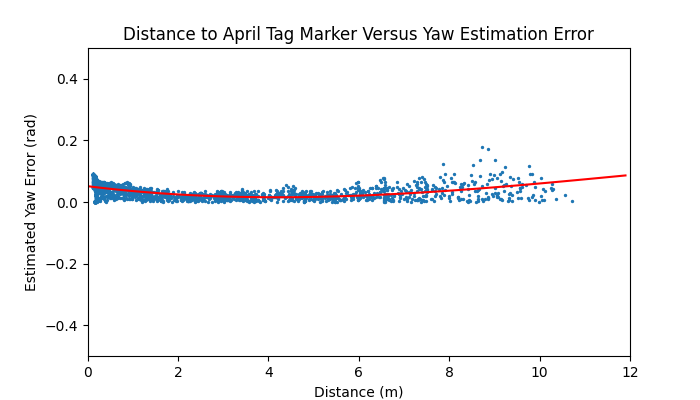
\includegraphics[width=0.65\textwidth]{images/apriltag_yaw_estimation_error.png}
    \caption{April Tag yaw estimation error with regression.}
    \label{fig:apriltag_yaw_estimation_error}
\end{figure}

The variance of the error in the April Tag's yaw estimation increases at very close distances. This is likely caused by the high angle of deflection of the marker in the camera's field of view, as shown by Figure \ref{fig:apriltag_landed_view}. However, this small issue can be overcome easily with the landing policy. The yaw position is locked if the yaw displacement of the drone is less than 5 degrees, or approximately 0.0873 radians, meaning that small variations in the yaw measurement will have no effect on the drone's behavior.

\begin{figure}[h]
    \centering
    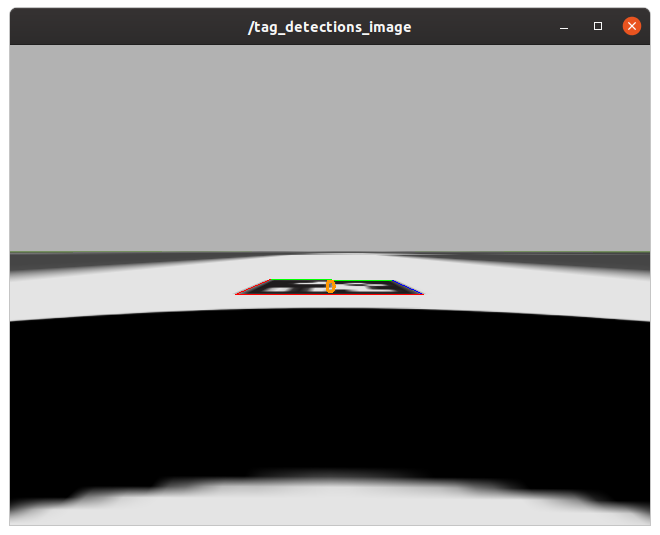
\includegraphics[width=0.5\textwidth]{images/landed_view.png}
    \caption{The view from the drone immediately after landing, with the April Tag's high angle of deflection.}
    \label{fig:apriltag_landed_view}
\end{figure}

% \section{\color{red}Landing Pad Pose Estimate Visualization}

% {\color{red}Here I will discuss an attempt to add a visualization for the landing pad pose estimate in Gazebo, the difficulties in using it, and why it was eventually abandoned.}


% \vspace{100cm}
\section{Initial PID Controller Tuning}
\label{subsection:pid_tuning}

% {\color{red}Here I will describe the process of tuning the velocity PID controllers. The intuitive way to describe it is that the distance at which the system changes from P to PD controllers, and the derivative gain were set to eliminate overshoot while minimizing the error over time. I still do not know exactly how to quantify this.}

PID controllers have parameters which must be tuned for the system and conditions that they will face. The first step in landing on a stationary platform is to tune these parameters using a priori knowledge of PID controller behavior and simple trial and error. Importantly, in a scenario involving a stationary landing platform with stable, well-tuned PID controllers, all of the state errors will converge to 0. This means that the integral gain of each of the PID controllers can be left at 0, making the control purely PD-based. This is conceptually different from a scenario wherein the landing pad is moving, which requires the additional integral gain (described in Section \ref{section:moving_landing_scenarios}). The approach taken in this project is to first tune the PID systems for a stable landing on a stationary landing platform, and then transition to moving landing scenarios, tuning only the integral gain.

\subsection{North and East Velocity Controllers}

The goals in tuning the gains of the east and north velocity PID controllers in order of priority are as follows:
\begin{enumerate}
    \item \textbf{Avoid overshoot.} Overshooting the landing platform causes complications in aiming the camera and increases both time and energy spent in landing.
    \item \textbf{Avoid undershoot.} Undershooting the landing platform increases the time and energy spent in landing. Avoiding overshoot takes precedence over avoiding undershoot. Overshoot is eliminated first. If this causes undershoot then the undershoot is gradually eliminated as long as it does not cause overshoot.
    \item \textbf{Minimize energy required for landing.} The energy required for landing must comprise only a small portion of the battery's capacity in order to maximize usable flight time for mission tasks. This metric is obviously related to the time spent for landing, but differs in that it accounts for energy-intensive maneuvers such as course correction.
    \item \textbf{Minimize time required for landing.} As the landing time increases, so does the possibility changes in the environment and the energy required for the landing.
\end{enumerate}

Initial, informal experiments showed that PID parameters shown in Table \ref{tab:initial_parameters} provided an imperfect but relatively reliable performance in the drone's approach towards the landing pad. These initial experiments decrease the search space for the PID parameters and therefore decrease the time for testing PID gains more rigorously. The parameters are all negative because the PID controllers in this scenario are reverse-acting - that is, a positive change in the control effort produces a negative change in the error between the set point and the state variable. Phase 1 refers to the PID gains used upon initial recognition of the landing platform. Phase 2 refers to the PID gains used when the drone is displaced by an intermediate distance from the landing platform. Phase 3 refers to the PID gains used when the drone is in its final approach.

\begin{table}[ht]
    \centering
    \begin{tabular}{|c|c|c|c|}
    \hline
        Phase & $k_p$ & $p_i$ & $k_d$ \\\hline
        1 & -0.7 & -0.0 & -0.4 \\\hline
        2 & -0.4 & -0.0 & -0.7 \\\hline
        3 & -0.3 & -0.0 & -0.9 \\\hline
    \end{tabular}
    \caption{Initial north and east PID tuning parameters. The same parameters are used for both systems.}
    \label{tab:initial_parameters}
\end{table}

The search space for the north and east PID parameters is comprised of all combinations of $k_p \pm 0.1$ and $k_d \pm 0.1$ for phases 1 and 2. The gains for phase 3 are kept constant in order to save time during the slow testing in Gazebo. Each of the combinations of gains is tested over 5 approaches. The approach series starts at the origin with an altitude of 10 meters, with the drone facing directly south in order to ensure that the landing platform is not in the drone's field of view. The landing controller is initially disabled by sending a PWM signal of 1100$\mu s$ on RC channel 11. Then, the drone is sent to a point 200 meters directly north of its original position, while also facing directly north. At this point, the landing controller is enabled by sending a PWM signal of 1900 $\mu s$ on RC channel 11. With each approach, the drone's starting position is moved 1 meter to the right in order to have variation in both planar dimensions of the drone's displacement from the landing pad. When the landing pad, positioned at 30 meters north of the origin, comes into the drone's field of view, the landing controller's north and east velocity PID controllers begin to control the drone. An approach is considered successful if the drone maintains a planar distance of no more than 1.6 meters from the landing pad (calculated through pose estimation) for 3 consecutive seconds. The system is given a maximum of 45 seconds from the acquisition of the landing platform to achieve a success before the approach is considered a failure. After a success or failure, the landing system is disabled, the drone is positioned at the starting point of the next approach, and the test is started again. For consistency, this process is automated using a Python script \texttt{control\_pid\_ne.py}. In this way, the drone follows exactly the same initial trajectory with the same velocity before acquisition of the landing platform. During these tests, the yaw correction and altitude correction of the landing system are inhibited to isolate the performance of the north and east PID controllers exclusively.

During each approach, the Python script records the time and energy required by the drone from the point of visual acquisition of the landing platform to a success or failure. The value for time is the ROS simulation time. The value for the energy is taken from the \texttt{battery\_status} MAVlink message 147. This message provides a value in \gls{hJ} given a properly calibrated power module onboard the drone. The gain combinations are rated according to the average time and energy required over the course of the 5 approaches. The 81 gain combinations are described by 405 separate approaches, but the results of the best combinations are shown in Table \ref{tab:initial_ne_gains}.

\begin{table}[h]
    \centering
    \begin{tabular}{|c|c|c|c|c|c|c|c|c|c|c|}
    	\hline $k_{p1}$ & $k_{i1}$ & $k_{d1}$ & $k_{p2}$ & $k_{i2}$ & $k_{d2}$ & $k_{p3}$ & $k_{i3}$ & $k_{d3}$ & $t_{ave}$ (s) & $e_{ave}$ (hJ) \\\hline
    	-0.7 & -0.0 & -0.4 & -0.3 & -0.0 & -0.7 & -0.3 & -0.0 & -0.8 & 13.0 & 52.4 \\\hline
    	-0.7 & -0.0 & -0.4 & -0.3 & -0.0 & -0.7 & -0.3 & -0.0 & -0.9 & 13.7 & 54.8 \\\hline
    	-0.7 & -0.0 & -0.4 & -0.3 & -0.0 & -0.8 & -0.3 & -0.0 & -0.9 & 13.8 & 55.4 \\\hline
    	-0.7 & -0.0 & -0.4 & -0.3 & -0.0 & -0.8 & -0.3 & -0.0 & -1.0 & 13.9 & 55.2 \\\hline
    	-0.7 & -0.0 & -0.4 & -0.3 & -0.0 & -0.8 & -0.2 & -0.0 & -0.8 & 15.0 & 60.0 \\\hline
    \end{tabular}
    \caption{Best 5 initial gain combinations by time and energy for the north and east PID controllers}
    \label{tab:initial_ne_gains}
\end{table}

\begin{figure}[ht]
    \centering
    % 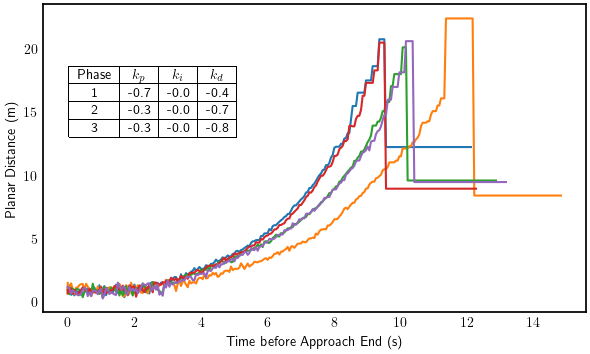
\includegraphics[width=0.45\textwidth]{images/best_initial_ne_pid_gains.png}
    % \caption{Caption}
    % \label{fig:my_label}
    \begin{subfigure}[b]{0.45\textwidth}
        \centering
        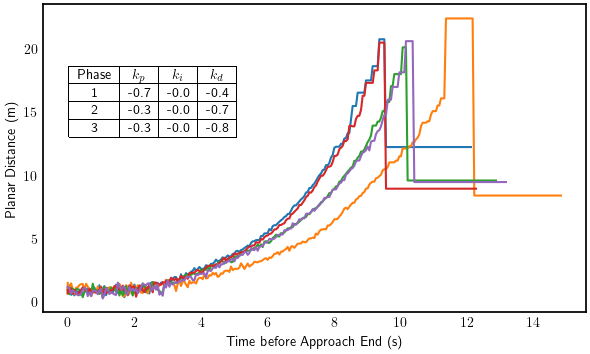
\includegraphics[width=\textwidth]{images/best_initial_ne_pid_gains.png}
        \caption{Best-performing N/E PID parameters.}
        \label{subfig:best_initial_pid_tuning}
    \end{subfigure}
    \begin{subfigure}[b]{0.45\textwidth}
        \centering
        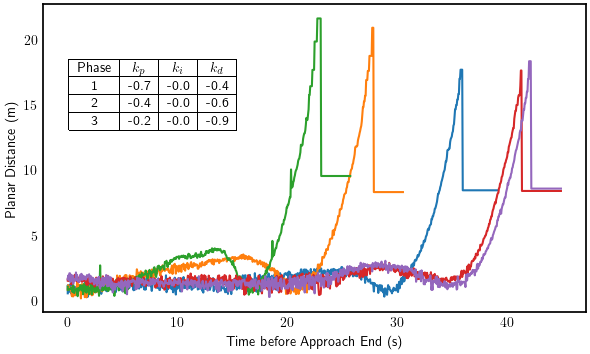
\includegraphics[width=\textwidth]{images/bad_ne_pid_tuning.png}
        \caption{Badly-performing N/E PID parameters.}
        \label{subfig:bad_initial_pid_tuning}
    \end{subfigure}
    \caption{Interesting initial north and east PID performances.}
    \label{fig:initial_ne_pid_gains}
\end{figure}

The graph of the best initial north and east PID gains is shown in Figure \ref{subfig:best_initial_pid_tuning}. The time plotted is the time \textit{before} a success or failure, so time $t=0$ indicates the point at which the drone's planar position has been sufficiently close to the landing platform's planar position for 3 seconds. The distance plotted is the difference in the planar positions of the drone and the landing pad. The perceived distance to the landing pad steadily and predictably decreases without salient local minima or maxima, which indicates that there is no positional overshoot. On the other hand, Figure \ref{subfig:bad_initial_pid_tuning} shows the performance of badly-performing PID parameters. Of the 5 approach attempts, only 3 were successful within the 45-second time limit, even with initial conditions which were negligibly different from those in Figure \ref{subfig:best_initial_pid_tuning}. Moreover, the salient local minima and maxima in the perceived distances shows that the drone approached the landing pad quickly, but overshot the target position and had to backtrack, which significantly increased the time and energy required for the approach. It is also important to note that these gains pertain to the most ideal scenario of landing on a stationary landing pad with no wind or other external factors.

Figure \ref{fig:initial_ne_pid_gains} additionally shows that the initial distance estimates (and inherently the initial pose estimates) of the drone relative to the landing platform are inaccurate. This means that the landing pad - the WhyCon marker in particular, since it is identified first - can be recognized in the drone's field of view before the pose can be accurately determined. This can be seen in all of the depicted approaches (and indeed in all of the test results) via the phenomenon that the initial distance estimate of about 10 meters, when the landing pad is just barely identifiable, jumps to about 18 meters when it becomes \textit{properly} identifiable. A number of factors are at play in causing this: namely the relatively small pixel area of the WhyCon marker within the drone's field of view, the angular displacement between the camera and the landing pad, and the motion of the camera as the gimbal controller attempts to aim the camera at the landing pad. A key aspect of the success of these tests is that the drone is moving towards the landing platform at the point when it is initially identified. This allows the pose estimation accuracy - and inherently the distance estimation accuracy - to increase over time.

\subsection{Up Velocity Controller}

The ``up'' PID controller is used to control the downward velocity of the drone during descent towards the landing platform. It is oriented upwards instead of downwards in order to conform to the typical east-north-up coordinate system orientation that is used in MAVROS and ArduPilot. As in the initial tuning for the north and east velocity PID controllers, the main goals in setting the initial gains for the velocity PID controller in the ``up'' direction are to prevent overshoot, prevent undershoot, and minimize time and energy spent. The most important of these goals is to prevent overshoot, as overshoot in this scenario means hitting the landing pad at higher than expected velocity.

Similarly to the north and east PID testing, the process of testing the up PID was automated by a Python script \texttt{control\_pid\_u.py}. The landing platform was positioned 30 meters directly north of the origin, and the drone was positioned directly above the landing platform at an altitude of 10 meters with the camera aimed directly at the landing platform and the landing controller disabled. At the point when the landing controller is enabled, a single test is considered to have begun, and the Python script records the position and velocity of the drone throughout the landing until the motors are disarmed. This is repeated for several sets of PD gains. The integral gain is not necessary here because the drone is not affected by persistent non-zero error in this dimension. The tests are repeated for all combinations of $k_p$ and $k_d$, where $k_p \in \{ 0.6, 0.7, 0.8, 0.9 \}$ and $k_d \in \{  0.4, 0.5, 0.6, 0.7 \}$. Each combination of gains is tested 5 times, giving a total of 80 runs. During these tests, the base descent radius is increased to 30 centimeters in order to avoid extraneous energy and time expenditure resulting from unavoidable drift in the drone's east and north positions. The best 5 gain combinations are shown in Table \ref{tab:up_pid_gains}.

\begin{table}[ht]
    \centering
    \begin{tabular}{|c|c|c|c|c|}
    	\hline $k_{p}$ & $k_{i}$ & $k_{d}$ & $t_{ave}$ (s) & $e_{ave}$ (hJ) \\\hline
    	-0.9 & -0.0 & -0.5 & 13.8 & 53.6 \\\hline
    	-0.8 & -0.0 & -0.4 & 13.8 & 54.0 \\\hline
    	-0.8 & -0.0 & -0.5 & 14.3 & 56.2 \\\hline
    	-0.9 & -0.0 & -0.7 & 14.4 & 56.0 \\\hline
    	-0.7 & -0.0 & -0.4 & 14.6 & 57.0 \\\hline
    \end{tabular}
    \caption{Best gain combinations for up velocity PID controller.}
    \label{tab:up_pid_gains}
\end{table}

Over the 80 tests, the average landing time for each combination is only in the range of $\left[ 13.8s, 19.7s \right]$, with a mean of $\mu_t = 16.06s$ and standard deviation of $\sigma_t = 3.14s$. The corresponding values for the energy expended are in the range $\left[ 53.6 \mathrm{hJ}, 73.4 \mathrm{hJ} \right]$, with mean $\mu_e = 61.75 \mathrm{hJ}$ and standard deviation $\sigma_e = 8.33 \mathrm{hJ}$. This means that the performances of all tested gain combinations are fairly similar, however the gains $k_p=-09, k_i=-0.0, k_d=-0.5$ are chosen according to the aforementioned goals. The performance of the best combination of gains is shown in Figure \ref{fig:best_u_pid_gains}.

\begin{figure}[ht]
    \centering
    \begin{subfigure}[b]{0.49\textwidth}
        \centering
        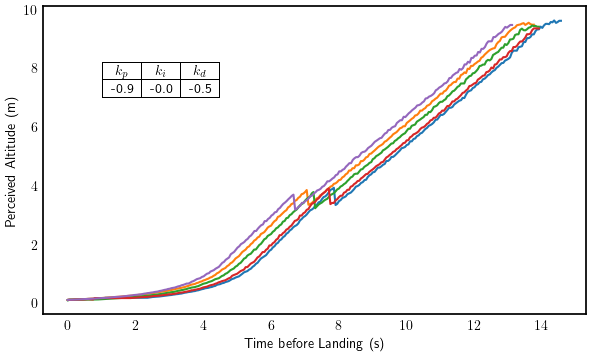
\includegraphics[width=\textwidth]{images/best_pid_u_altitude.png}
        \caption{Perceived altitude vs. time before landing.}
        \label{subfig:best_initial_pid_u_altitude}
    \end{subfigure}
    \begin{subfigure}[b]{0.49\textwidth}
        \centering
        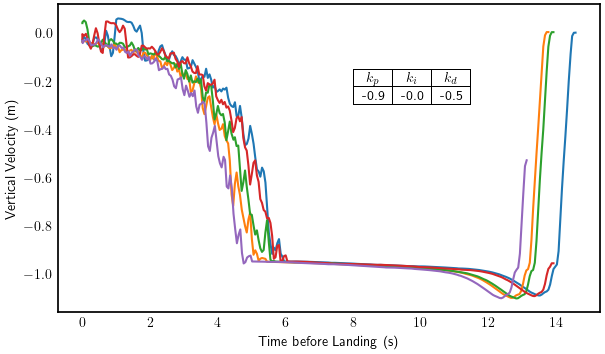
\includegraphics[width=\textwidth]{images/best_pid_u_velocity.png}
        \caption{Vertical velocity vs. time before landing.}
        \label{subfig:best_initial_pid_u_velocity}
    \end{subfigure}
    \caption{Visualization of best U PID gain performance.}
    \label{fig:best_u_pid_gains}
\end{figure}

Figure \ref{subfig:best_initial_pid_u_altitude} shows the near-linear descent of the drone towards the landing platform in the early part of the landing, with a gradual slowdown as the drone gets closer and closer to touchdown. Figure \ref{subfig:best_initial_pid_u_velocity} shows the same phenomenon in terms of velocity. The magnitude of the velocity increases suddenly after the landing controller is enabled, then remains relatively constant until the derivative component of the PID system slows the velocity to 0.

\subsection{Yaw Velocity Controller}

The gains for the yaw velocity controller were determined experimentally through tests similar to those for the other PID controllers. Specifically, the test is automated using a Python script \texttt{control\_yaw\_testing.py}. First, the drone is positioned directly above the landing pad at an altitude of 10 meters. With the landing controller disabled, the drone rotates to 10 different initial angles which are equally placed in the interval $\theta_{initial} \in [0, 2\pi)$. The landing controller is then enabled, with the linear velocity set points always equal to 0, in order to isolate the behavior of the yaw PID controller. The time and yaw displacement are recorded for 10 seconds. The process is repeated at the same location for the remaining initial angles. The entire process is then repeated for multiple positions.

Since the Iris model has very accurate control over its yaw position and velocity, the yaw velocity PID controller performs very well. The results are illustrated in Figure \ref{fig:initial_yaw_tuning}.

\begin{figure}[ht]
    \centering
    \begin{subfigure}[b]{0.45\textwidth}
        \centering
        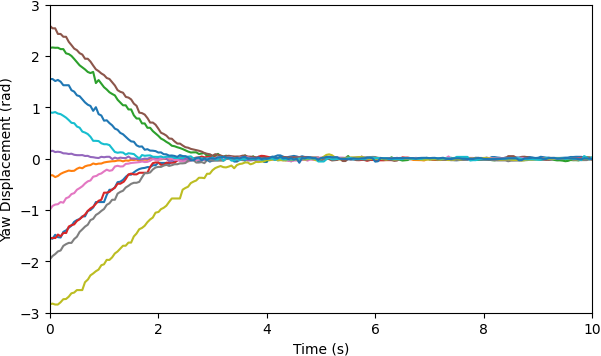
\includegraphics[width=\textwidth]{images/yaw_pid_testing_east_0.png}
        \caption{Yaw correction with drone directly above landing pad at altitude of 10 meters.}
        \label{subfig:yaw_pid_testing_east_0}
    \end{subfigure}
    \begin{subfigure}[b]{0.45\textwidth}
        \centering
        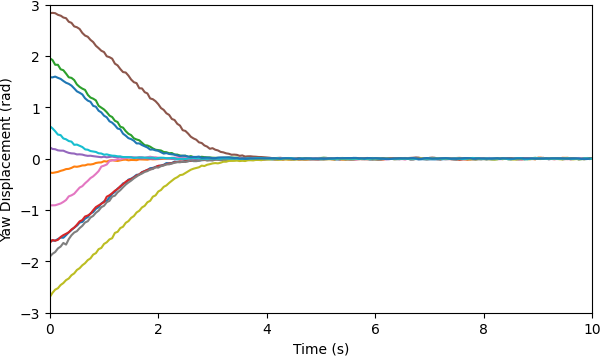
\includegraphics[width=\textwidth]{images/yaw_pid_testing_east_2.png}
        \caption{Yaw correction with drone 2 meters east of landing platform at altitude of 7 meters.}
        \label{subfig:yaw_pid_testing_east_2}
    \end{subfigure}
    \caption{Visualization of velocity yaw controller performance.}
    \label{fig:initial_yaw_tuning}
\end{figure}

\section{Stationary Landing Scenarios}
\label{subsection:stationary_landing_scenarios}

The first test of the landing system in its entirety is a series of 5 landing sequences starting with the drone at the origin and the landing platform 30 meters directly north of the origin. These are essentially a repeat of the test for the north and east velocity PID systems, but with the up and yaw PID systems active. The results for the initial gains are visualized in Figure \ref{subfig:linear_land_test_initial}. After initial descent, it is easy to see a sharp inflection point representing positional overshoot overshoot. Although the parameters do allow the system to land successfully, the overshoot is not ideal. The system parameters were re-tuned manually over the course of several experiments. The descent region was slightly enlarged, giving the drone more area to continue its descent without stopping, and causing earlier PID reconfiguration. The derivative gain $k_d$ was increased in phases 2 and 3 in order to slow the drone more drastically. The proportional gain was decreased in phase 2, also to slow the drone's approach. The resulting, smoother performance is shown in Figure \ref{subfig:linear_land_test_better}, and the performances are compared in Table \ref{tab:linear_land_performance_comparison}.

\begin{figure}[ht]
    \centering
    \begin{subfigure}[b]{0.45\textwidth}
        \centering
        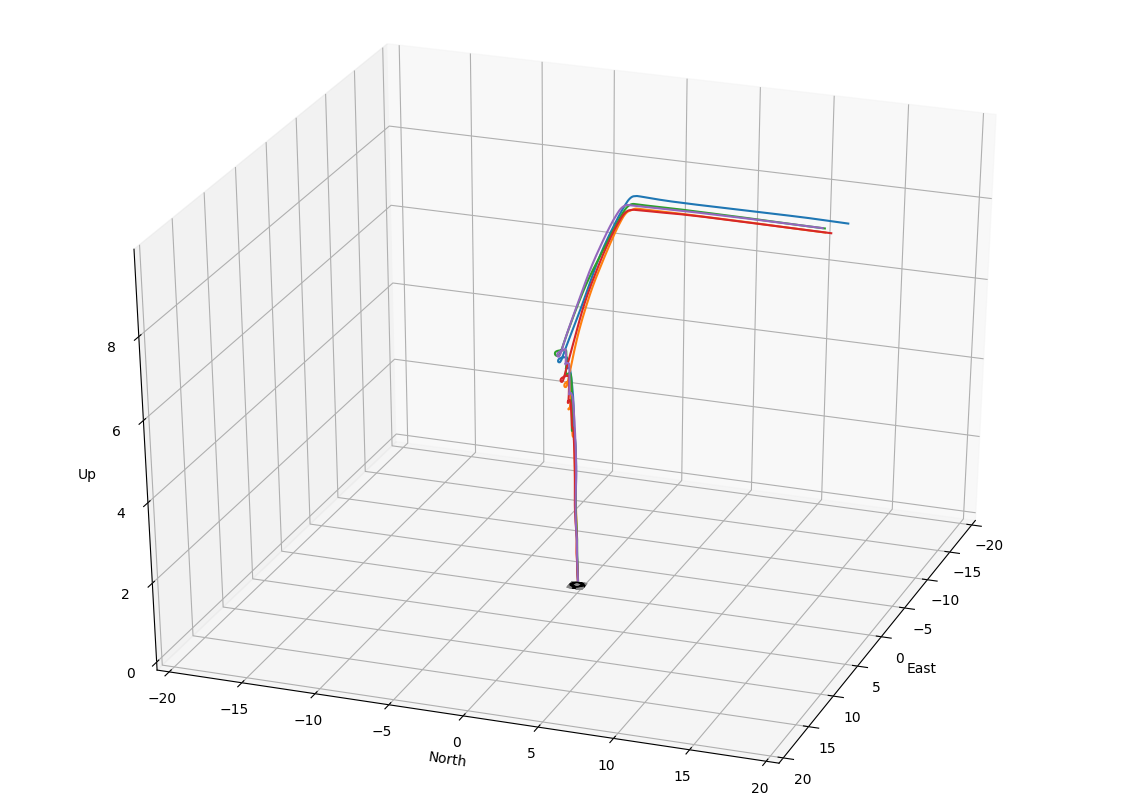
\includegraphics[width=\textwidth]{images/linear_land_test_initial.png}
        \caption{Initial parameters (positional overshoot).}
        \label{subfig:linear_land_test_initial}
    \end{subfigure}
    \begin{subfigure}[b]{0.45\textwidth}
        \centering
        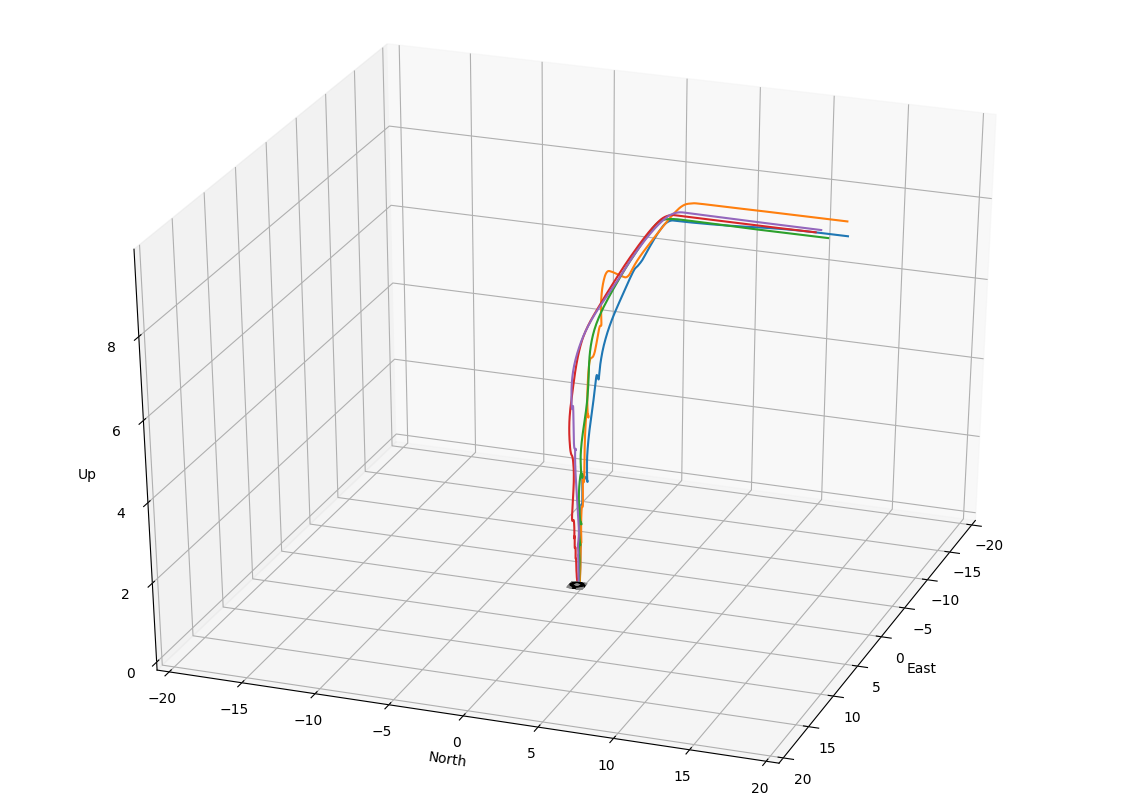
\includegraphics[width=\textwidth]{images/linear_land_test_better.png}
        \caption{Looser, more efficient parameters.}
        \label{subfig:linear_land_test_better}
    \end{subfigure}
    \caption{Comparison of initial parameters versus manually-tuned parameters.}
    \label{fig:initial_u_pid_gains}
\end{figure}

\begin{table}[ht]
    \centering
    \resizebox{\textwidth}{!}
    { 
    \begin{tabular}{|c|c|c|c|c|c|c|c|c|c|c|c|c|c|}
    \cline{2-14}
    	\multicolumn{1}{c|}{} & $k_{p1}$ & $k_{i1}$ & $k_{d1}$ & $k_{p2}$ & $k_{i2}$ & $k_{d2}$ & $k_{p3}$ & $k_{i3}$ & $k_{d3}$ & $\mu_t$ (s) & $\sigma_t$ (s) & $\mu_e$ (hJ) & $\sigma_e$ (hJ) \\\hline
    	Initial & -0.7 & -0.0 & -0.4 & -0.3 & -0.0 & -0.7 & -0.3 & -0.0 & -0.8 & 39.8 & 0.65 & 130.0 & 2.1 \\\hline
    	Improved & -0.7 & -0.0 & -0.4 & -0.3 & -0.0 & -0.8 & -0.3 & -0.0 & -0.9 & 35.6 & 1.8 & 112.8 & 7.5 \\\hline
    \end{tabular}
    }
    \caption{Comparison of initial and manually-tuned gains and performances during 5 linear landing tests.}
    \label{tab:linear_land_performance_comparison}
\end{table}

Figure \ref{subfig:radial_land_test_initial} represents the landing trajectories taken by the drone over a series of 10 landings from various angles around the landing platform using the initially-determined PID gains and system parameters. Gazebo provides the coordinates of the Iris model via a ROS topic and these are used as a true value for the position of the drone. The landing pad is positioned at $(x,y,z)=(0,30,0)$ in the ENU coordinate frame starting at the origin of \texttt{sandbox.world}. For clarity, the plotted trajectories begin at the moment that the drone first detects the landing pad and continue until the drone has landed. The approaches begin at a height of 10 meters. A Python script places the drone initially in 10 equidistant starting points which are positioned around the landing pad at a radius of 30 meters. The landing controller is then enabled and the drone is sent towards the landing pad. Upon detection of the landing pad, the landing controller takes control of the drone until it lands and disarms, at which point the drone begins another landing test at the next starting point.

\begin{figure}[ht]
    \centering
    \begin{subfigure}[b]{0.45\textwidth}
        \centering
        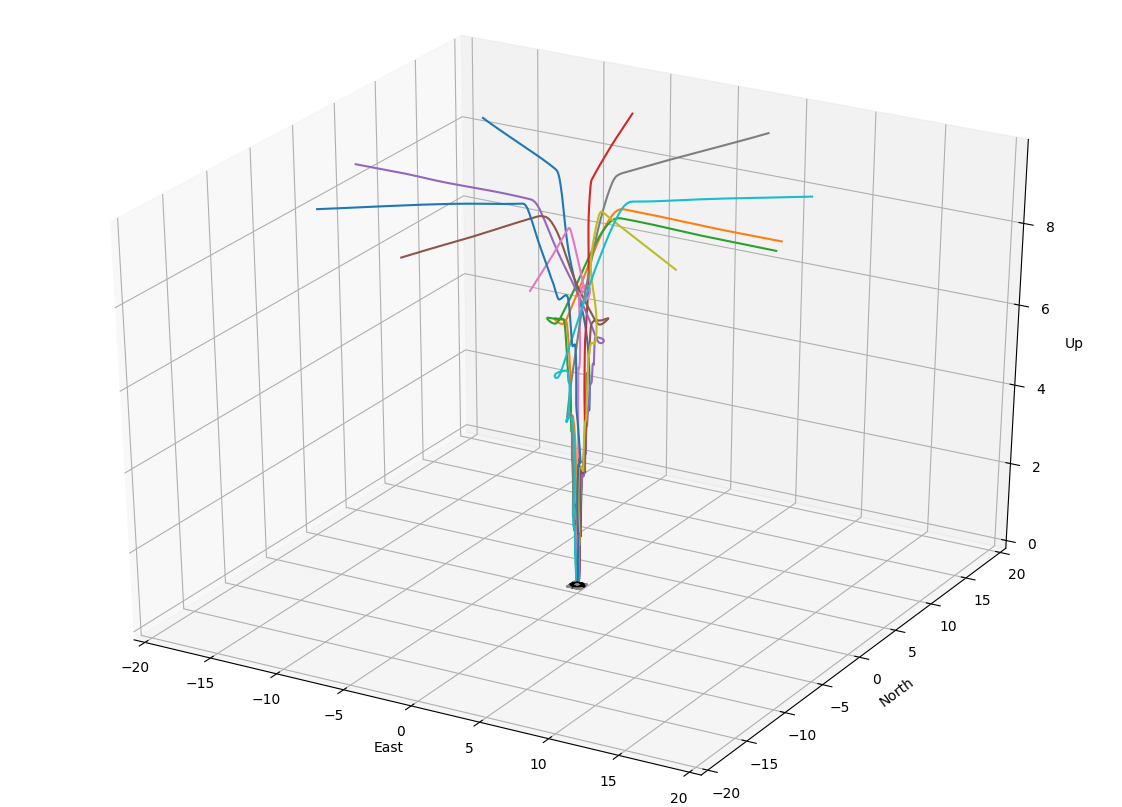
\includegraphics[width=\textwidth]{images/radial_land_test_initial.png}
        \caption{Initial parameters (positional overshoot).}
        \label{subfig:radial_land_test_initial}
    \end{subfigure}
    \begin{subfigure}[b]{0.45\textwidth}
        \centering
        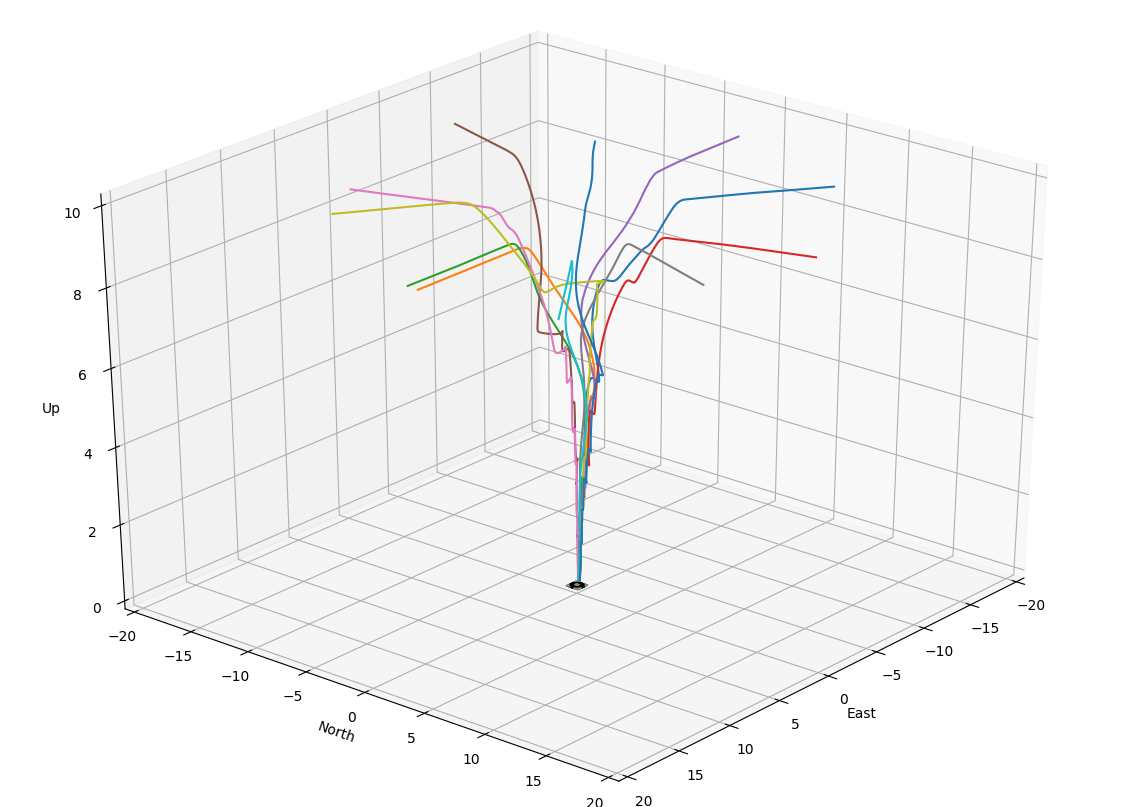
\includegraphics[width=\textwidth]{images/radial_land_test_better.png}
        \caption{Looser, more efficient parameters.}
        \label{subfig:radial_land_test_better}
    \end{subfigure}
    \caption{Radial landing tests.}
    \label{fig:radial_land_test_better}
\end{figure}

\begin{table}[ht]
    \centering
    \begin{tabular}{|c|c|c|c|c|}
    \cline{2-5}
    	\multicolumn{1}{c|}{} & $\mu_t$ & $\sigma_t$ & $\mu_e$ & $\sigma_e$ \\\hline
    	Initial & 37.5 & 3.06 & 120.5 & 12.2 \\\hline
    	Improved & 36.8 & 4.38 & 117.8 & 17.3 \\\hline
    \end{tabular}
    \caption{Caption}
    \label{tab:my_label}
\end{table}

A key result from this test is that the landing trajectories are not completely smooth, particularly in the cases where the drone's yaw is significantly different from that of the landing platform. This is because, when the drone orients its yaw to that of the landing platform, the drone's angular velocity means that the PID control efforts in the north and east direction are not fully aligned to the landing pad. This causes the drone to drift slightly out of the descent region, stopping the descent and giving the drone more time to correct its position. However, in all cases, the drone lands successfully.

Figure \ref{fig:initial_landing_trajectories_estimate} shows the trajectories of these same landings from the point of the view of the drone's pose estimation system. The perceived positive displacement in the north direction, and small perceived displacement in the east direction describe the fact that the drone is approaching the landing platform head-on.

\begin{figure}[ht]
    \centering
    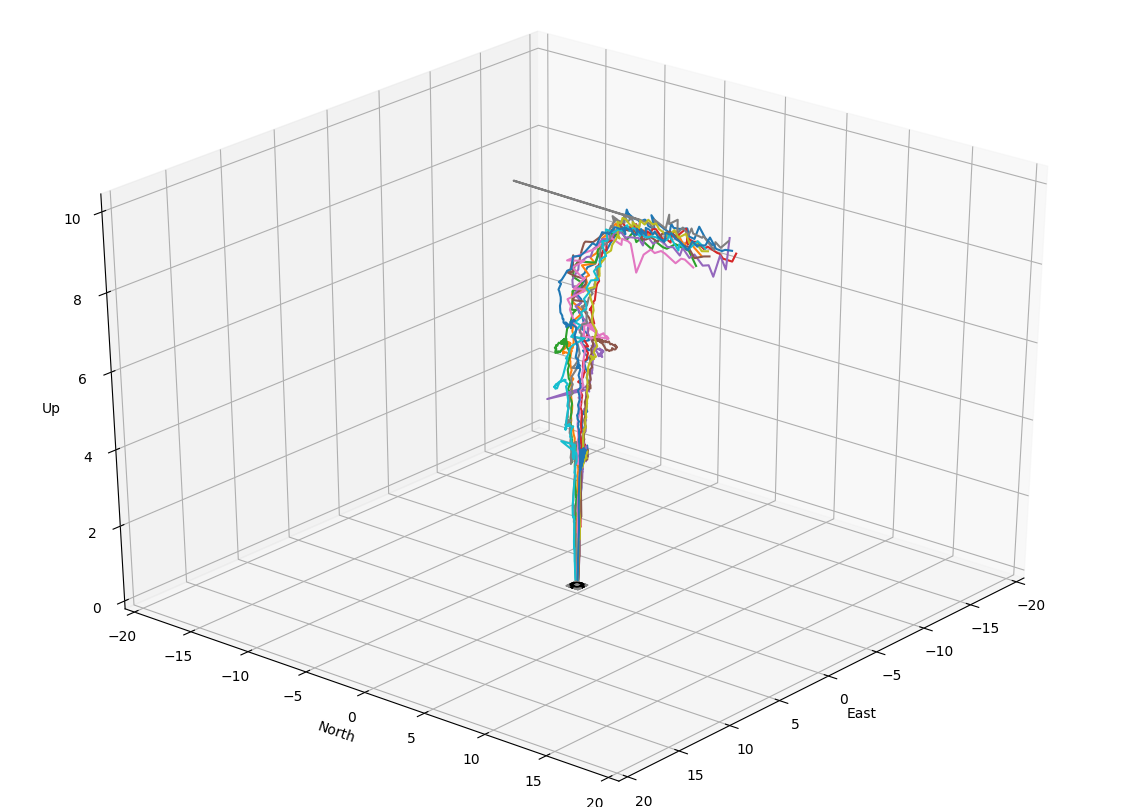
\includegraphics[width=0.7\textwidth]{images/initial_landing_trajectories_estimate.png}
    \caption{Estimated trajectories of the initial landing sequences with respect to the drone's position and orientation.}
    \label{fig:initial_landing_trajectories_estimate}
\end{figure}

The descent region for this series of landings is defined using Equation \ref{equation:plane_distance_threshold} with $k_1=0.12$ and $k_2=0.36$ in order to allow for descent starting at a planar distance of about 4.4 meters from the landing pad when the drone is at an altitude of 10 meters. This does mean that the drone is still allowed to descend when displaced by up to 0.12 meters from the center of the landing pad at an altitude of 0 meters. These constraints can be changed to suit the conditions of the landing pad and the performance of the drone.

% \begin{figure}[ht]
%     \centering
%     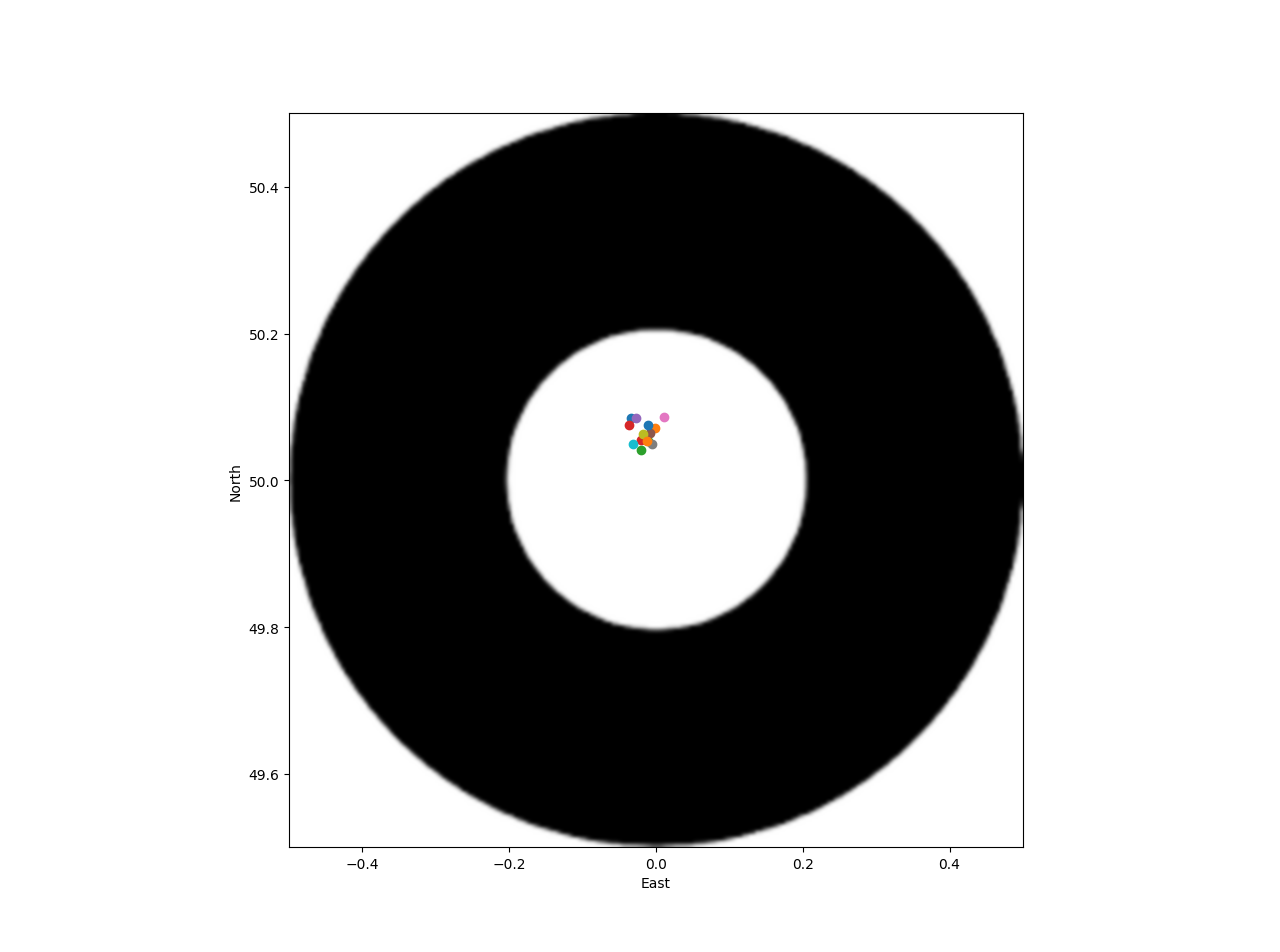
\includegraphics[width=\textwidth]{images/landing_points_of_contact.png}
%     \caption{Points of contact with the landing pad for the landing trajectories shown in Figure \ref{fig:landing_trajectories}}
%     \label{fig:points_of_contact}
% \end{figure}

% \newpage
\section{Moving Landing Scenarios}
\label{section:moving_landing_scenarios}

In order to test the landing system in the context of a moving landing platform, a test similar to the stationary linear landing tests was carried out. A Python script \texttt{control\_moving\_landings.py} automates this process. The drone is first positioned at the origin at an altitude of 10 meters, with a yaw of -1.6 radians (meaning that it is pointed directly south with the landing system disabled. The landing platform is positioned 30 meters directly north of the origin. The drone is then sent to a point 200 meters north of the origin, facing at a yaw position of 1.6 radians (directly north), with the landing system enabled. Before the drone identifies the landing platform, the landing platform begins to move directly north at a given speed which is specific to each test. The time, positions of the drone and landing platform, energy consumed, and the pose estimate of the landing platform relative to the drone are recorded from the moment that the drone recognizes the landing platform. When the drone recognizes the landing platform, the landing controller takes control and directs the drone to land on the moving landing platform. The test stops when ArduPilot detects the landing and automatically disarms the motors, at which point the drone returns to its original position and orientation at the origin, the landing platform is sent to its original position and orientation, and the test begins again. Figure \ref{fig:moving_land_testing_1mps} visualizes the trajectory of the drone relative to the landing pad over the course of 5 landings wherein the drone is moving at a constant velocity of 1 $\frac{m}{s}$. 

% \begin{figure}
%     \centering
%     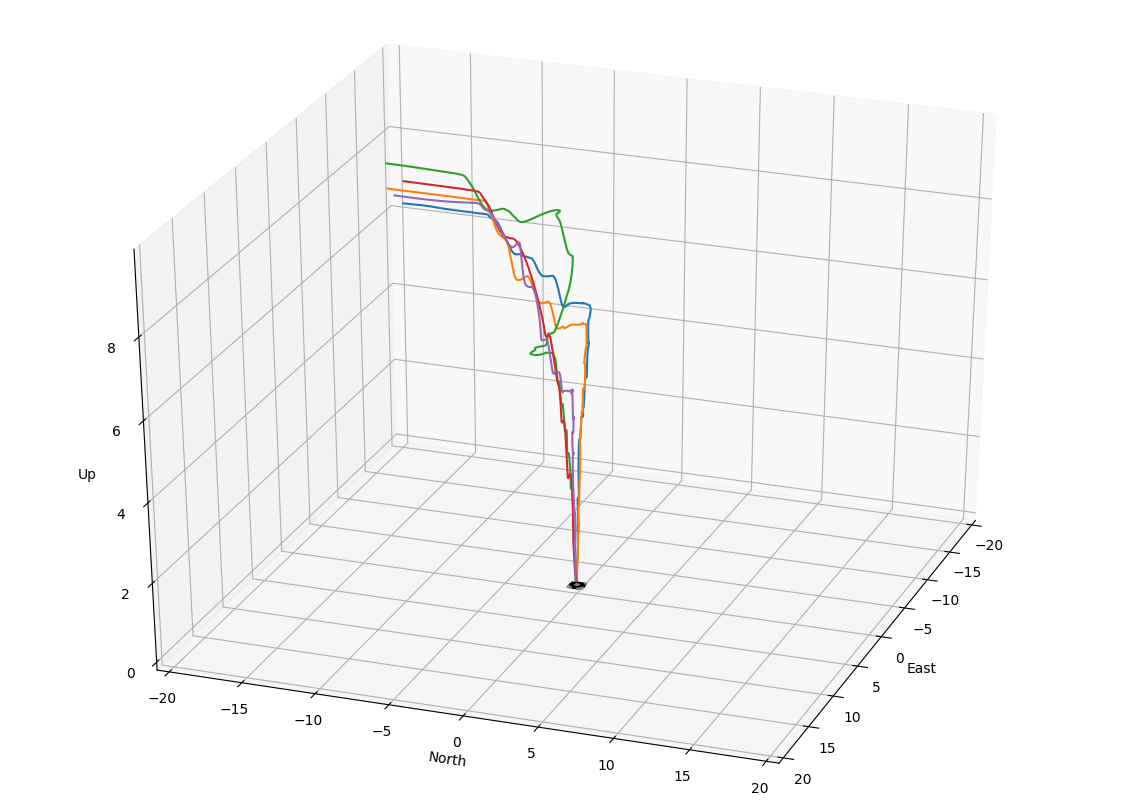
\includegraphics[width=0.75\textwidth]{images/moving_land_testing_1mps.png}
%     \caption{Relative landing trajectory for a moving landing at 1 $\frac{m}{s}$}
%     \label{fig:moving_land_testing_1mps}
% \end{figure}

\begin{figure}[ht]
    \centering
    \begin{subfigure}[b]{0.49\textwidth}
        \centering
        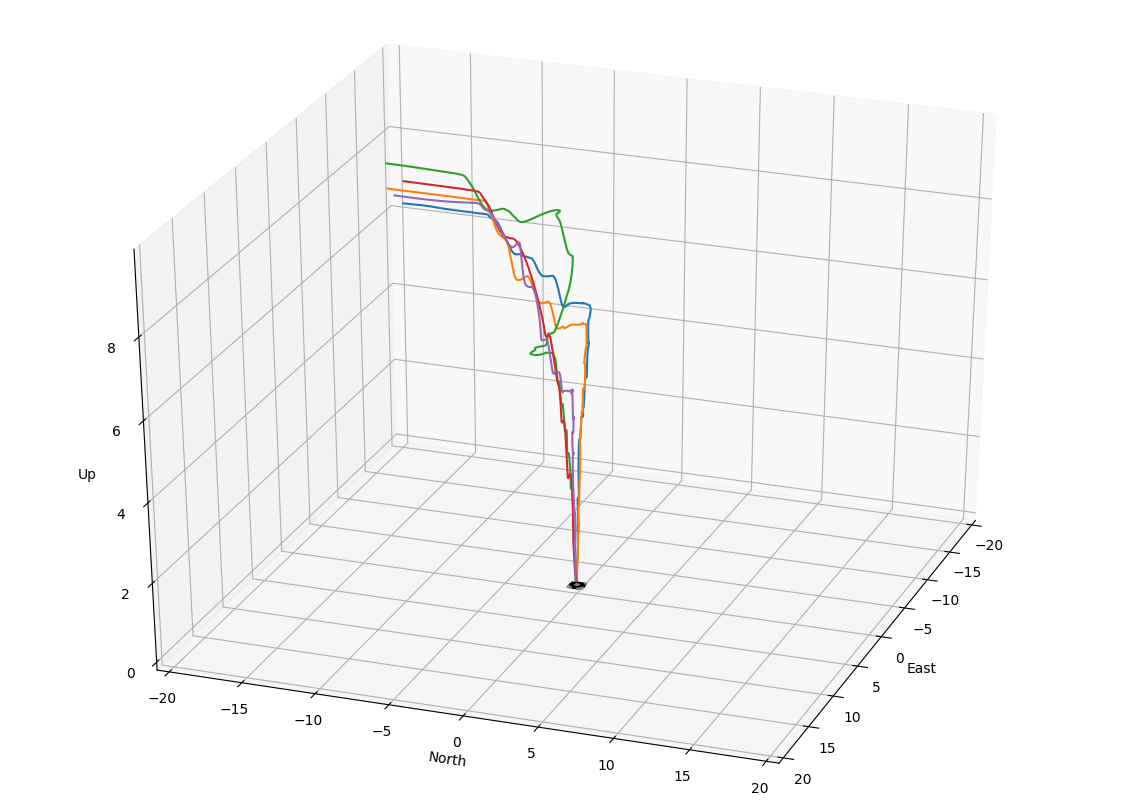
\includegraphics[width=\textwidth]{images/moving_land_testing_1mps.png}
        \caption{Relative landing trajectory.}
        \label{subfig:moving_land_testing_1mps_relative}
    \end{subfigure}
    \begin{subfigure}[b]{0.49\textwidth}
        \centering
        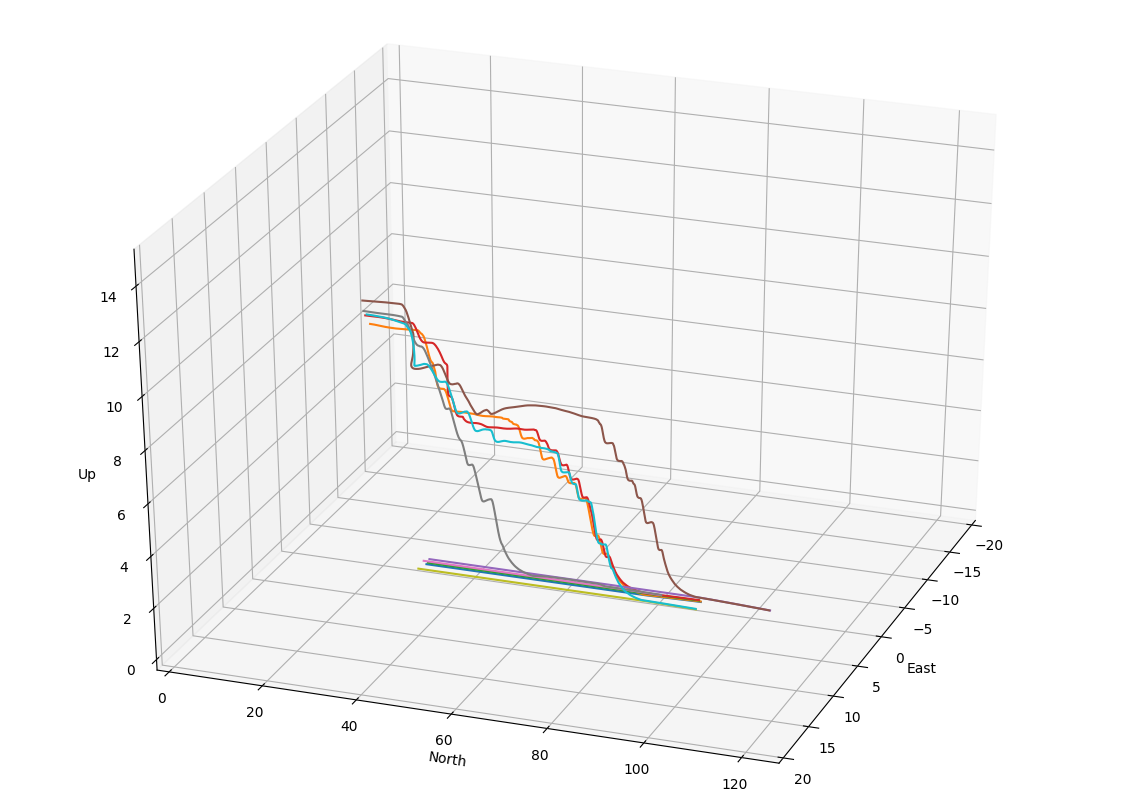
\includegraphics[width=\textwidth]{images/moving_land_testing_1mps_absolute.png}
        \caption{Absolute landing trajectory.}
        \label{subfig:moving_land_testing_1mps_absolute}
    \end{subfigure}
    \caption{Moving land tests with landing platform speed 1 $\frac{m}{s}$}
    \label{fig:moving_land_testing_1mps}
\end{figure}

\begin{figure}[ht]
    \centering
    \begin{subfigure}[b]{0.49\textwidth}
        \centering
        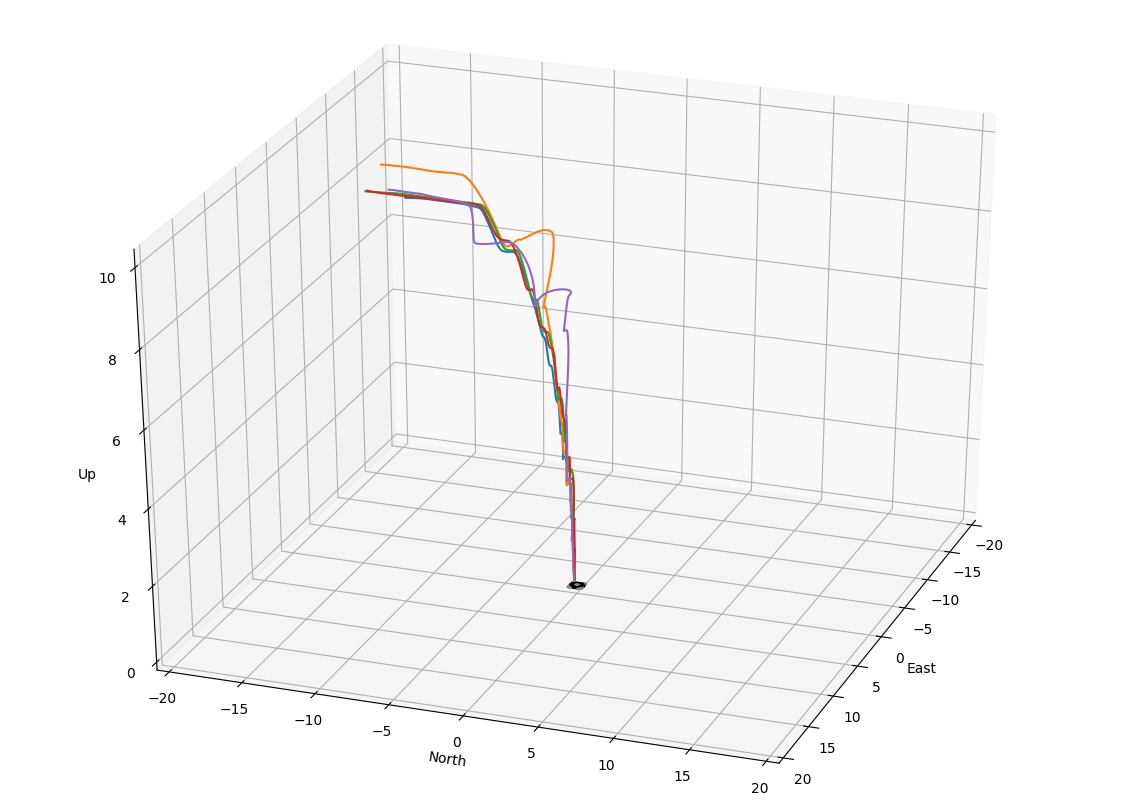
\includegraphics[width=\textwidth]{images/moving_land_testing_5mps.png}
        \caption{Relative landing trajectory.}
        \label{subfig:moving_land_testing_5mps_relative}
    \end{subfigure}
    \begin{subfigure}[b]{0.49\textwidth}
        \centering
        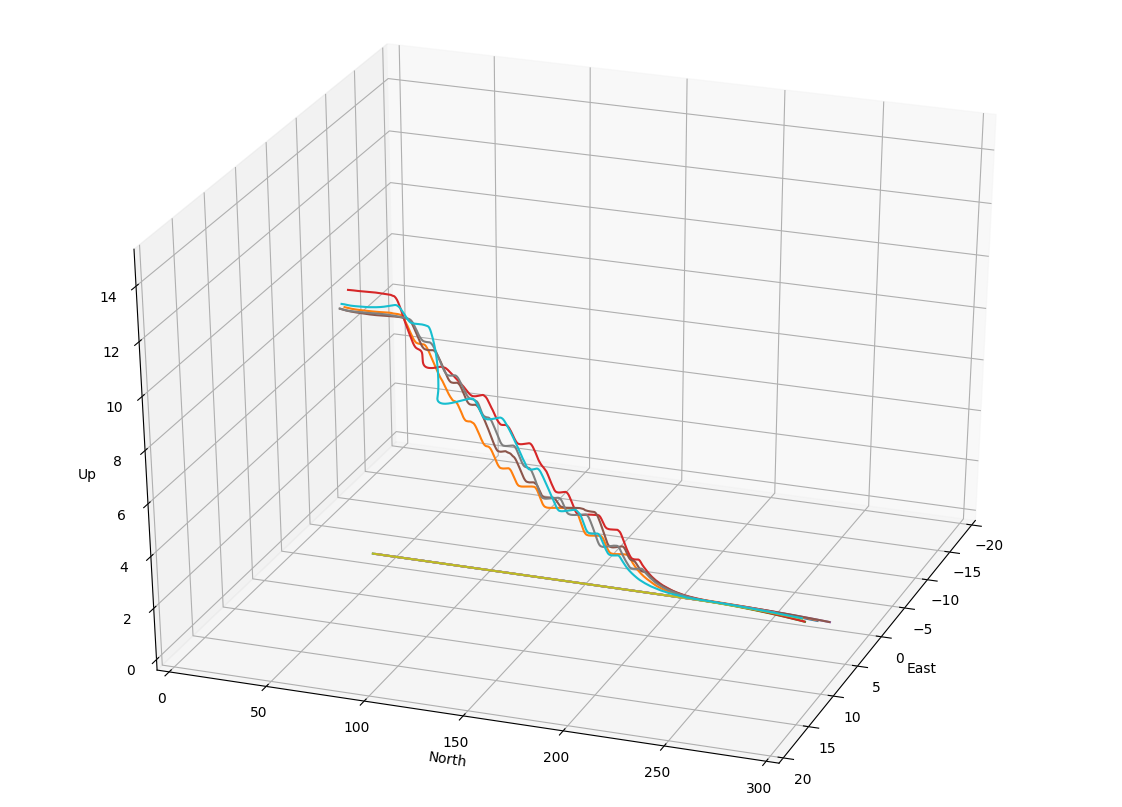
\includegraphics[width=\textwidth]{images/moving_land_testing_5mps_absolute.png}
        \caption{Absolute landing trajectory.}
        \label{subfig:moving_land_testing_5mps_absolute}
    \end{subfigure}
    \caption{Moving land tests with landing platform speed 5 $\frac{m}{s}$}
    \label{fig:moving_land_testing_5mps}
\end{figure}

For landing at 1 $\frac{m}{s}$, the north and east velocity PID controllers required an integral gain of $k_i=0.22$ in the last phase of landing. The landings required 61.09 seconds and 213.6 hJ on average. As shown in Figure \ref{subfig:moving_land_testing_1mps_relative}, the drone initially recognized the landing platform at a planar distance of about 15 meters away, at an altitude of 10 meters. Figure \ref{subfig:moving_land_testing_1mps_absolute} shows the distance over which the drone executed the landing, which was about 60.89 meters - consistent with the time required when considering that the landing pad was moving at 1 $\frac{m}{s}$. Figure \ref{fig:moving_land_testing_5mps} shows a similar test, with the landing platform moving at a speed of 5 $\frac{m}{s}$. The landings required 45.22 seconds and 159.8 hJ on average. The better performance is likely due to the fact that $k_i$ was set to 0.1 in both phases 2 and 3, which allowed for a generally smoother descent than in the 1 $\frac{m}{s}$ test, where $k_i$ was 0 in phase 2. The PD control in phase 2 meant that the integral component of the control effort started increasing only in phase 3. This slowly-increasing, long-term integral effect should be considered in tuning the velocity PID controllers in a physical system. 

\section{Radial Landings in Wind}
\label{section:radial_landings_wind}

The ArduPilot Gazebo repository provides a plugin for simulating changing wind, which was leveraged in order to see the resulting change in behavior of the drone during landing, which is especially important in real-world landing scenarios where wind will always be present. Another radial landing test was carried out in the presence of wind. The horizontal components of the wind are biased with base velocities of 1 $\frac{m}{s}$ in both the north and west directions. A sine function with an amplitude of 1 $\frac{m}{s}$ and a period of 20 seconds changes the magnitude continuously. Gaussian noise with a mean of 1 $\frac{m}{s}$ and standard deviation of 0.5 $\frac{m}{s}$ is also added. The direction of the of the wind also changes over time with both a sine function with amplitude 1 rad and a period of 10, as well as with Gaussian noise with a mean of 1 rad and standard deviation of 0.5 rad. Figure \ref{fig:radial_landings_wind} shows the trajectories of the drone during this test, required 40.7 seconds and 137.5 hJ on average. 

\begin{figure}[ht]
    \centering
    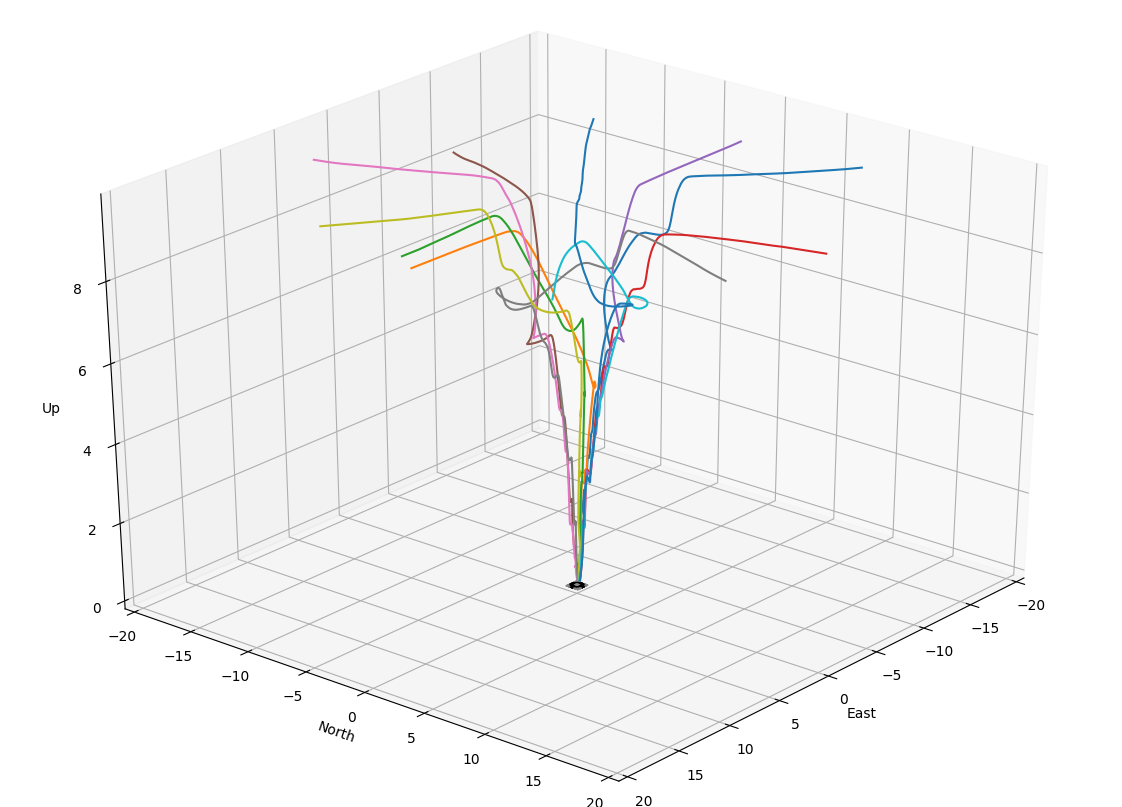
\includegraphics[width=0.6\textwidth]{images/randial_land_testing_wind.png}
    \caption{Trajectories of the drone relative to the landing platform over 11 landings with wind.}
    \label{fig:radial_landings_wind}
\end{figure}

It was necessary and beneficial to add a small integral gain of $k_i=-0.01$ in phase 3 in order to overcome the persistent error caused by the biased wind. This is representative of a real world scenario. It was also necessary to increase the size of the descent region at lower altitudes. The constants $k_1$ and $k_2$ from Equation \ref{equation:plane_distance_threshold} were set to 0.24 and 0.36. Additionally, the high wind caused the drone to have a biased attitude in order to maintain its position over the landing pad. This did not prohibit landing, but it did mean that not all of the legs of the drone made contact with the landing pad at the same time. To minimize the effects of this, the altitude at which the drone committed to the landing and dropped to the landing platform was increased from 9 cm to 14 cm. This is important because, if some but not all of the legs are touching the landing platform, the degrees of freedom of the drone are reduced. This reduces the ability of the drone to control its attitude - and therefore its velocity as well. The time during which the drone experiences this reduction in its freedom of movement must be minimized in order to guarantee a stable landing.